\documentclass{article}
\usepackage{fullpage}
\usepackage{amsmath,amssymb,amsthm}
\usepackage[hidelinks]{hyperref}
\usepackage{graphicx}
\usepackage[utf8]{inputenc}
\usepackage{xcolor}
\usepackage{natbib}

\bibliographystyle{plainnat}

\newcommand{\comdist}{\widetilde{R}}
\newcommand{\comdistfn}{\widetilde{\mathcal{R}}}

\newcommand{\R}{\mathbb{R}}
\newcommand{\norm}[1]{\left\lVert#1\right\rVert}
\DeclareMathOperator{\var}{\mathop{\mbox{Var}}}
\DeclareMathOperator{\cov}{\mathop{\mbox{Cov}}}
\DeclareMathOperator{\diag}{\mathop{\mbox{diag}}}

\renewcommand{\P}{\mathbb{P}}
\newcommand{\E}{\mathbb{E}}
\newcommand{\given}{\,\vert\,}
\newcommand{\supp}{\mathop{\mbox{supp}}}
\newcommand{\sgn}{\mathop{\mbox{sgn}}}
\newcommand{\EE}[1]{\E\!\left[#1\right]}
\newcommand{\PP}[1]{\P\!\left\{#1\right\}}
\newcommand{\PPP}[2]{\P_{#1}\!\left\{#2\right\}}
\newcommand{\EEE}[2]{\E_{#1}\!\left[#2\right]}
\newcommand{\EEsup}[2]{\E^{#1}\!\left[#2\right]}

\newcommand{\bone}{\mathbf{1}}

\newcommand{\plr}[1]{{\em \color{blue} #1}}

\begin{document}

\title{Are populations like a circuit? The relationship between isolation by distance and isolation by resistance}
\author{Erik Lundgren\footnote{Computational Biology, University of Southern California}, and
        Peter L. Ralph\footnote{Institute for Ecology and Evolution, University of Oregon}}
\maketitle

\begin{abstract}
\plr{abstract needs editing}
A number of methods commonly used in landscape genetics
use analogies to electrical resistance on a network
to describe and fit barriers to movement across the landscape
using genetic distance data.
These are motivated by a mathematical eqiuvalence of effective resistance
to the mean commute time of a random walk.
Here, we describe the differences between commute time
and coalescence time, which more accurately models genetic distances,
and explore the consequences for inference.
We implement a Bayesian method to do inference under both these models,
and find that inference using commute times
when the data derive from coalescence times
can dramatically mislead in the presence of biased gene flow.
We apply the methods to empirical data,
and find evidence for strongly biased gene flow.
\end{abstract}


%%%%%%%%%%%%%%%%%%%%%%
\section*{Introduction}

Genetic relatedness is determined by past gene flow,
a product of individual or gamete movements across geographic space.
Genomes therefore retain the traces of this movement,
and can contribute to the inference of how a species moves across a landscape,
which is important for understanding how diseases spread, how species adapt,
and how to retain genetic diversity in threatened species.
This is a potentially important source of information,
as direct observation can be difficult \citep[especially of long-distance movement]{dispersal_estimation},
or even impossible, if some of the populations in question no longer exist.

The idea of ``resistance distance'' is an important tool in the lanscape genomics toolbox.
Introduced by \citet{mcrae2006isolation},
it makes use of a mathematical equivalence between random walks and electrical resistance
\citep{resistance}:
the expected time for a continuous-time Markov chain that starts at node $x$
to first hit node $y$ and then return to $x$ (the ``commute time'')
is equal to the effective resistance between $x$ and $y$ in an electrical network
whose conductances are given by the movement rates of the Markov chain \citep{levin}.
This measure therefore averages over all possible paths through the network between the two.
For this reason, 
if assigning local conductances based on the values of some landscape variable
results in a significant positive correlation between 
genetic distances between samples from different parts of the landscape
and the effective resistances between those locations,
then this is taken as good evidence that the landscape variable is a good indicator of
where gene flow occurs \citep{mcrae2007circuit,cushman2006complex,more_examples}.
For instance,
if the conductance across a grid cell in a discretization of the landscape
is higher in flatter areas,
and this produces effective resistance values 
that are significantly correlated with genetic distances,
then one might conclude that the species in question tends to disperse more readily through flatter areas,
perhaps along river valleys.
More recent methods \citep{petkova2016visualizing,hanks2013circuit} seek to build \emph{de novo} 
a map of conductance values that produces resistances 
most strongly correlated with observed genetic distance,
and then interpret regions of low conductance in the resulting map as barriers to gene flow.

As motivated by \citet{mcrae2006isolation},
commute time (i.e., resistance distance) is a more computationally tractable approximation
to \emph{coalescence time}, a more accurate model of genetic distance data.
Genetic distances between two genomes sampled from the landscape
do derive from an average across a large number of paths between those points --
the lineages along which each segment of genetic material has been inherited
from their most recent common ancestor.
The more recent this ancestor is,
the smaller the genetic distance will be.
Thanks to recombination, there are a large number of such paths, 
and genetic distance averages over these.
It is reasonable in some situations to model these lineages as random walks across the landscape;
however, the model of genetic distance that one is thus led to
is \emph{coalescence time} of the random walks, 
rather than commute time, the quantity that corresponds to resistance.
This naturally raises the question: 
Are methods that depend on effective resistances being misled?
If so, would using coalescence time do better?

\citet{mcrae2006isolation} showed that coalescence time and resistance distance are equal
(up to shift and scaling) in isotropic landscapes such as a ring \citep{matsen_wakeley},
and found that the two were highly correlated in several test cases.
However, all these test cases involved symmetric rates of gene flow,
which is likely not the case in many situations, e.g.,
in rivers \citep{morrissey2009maintenance,sundqvist2016directional,hanks2017modeling},
source-sink dynamics \citep{source_sink},
or after population expansions \citep{expansions}.

\plr{CHANGE TO mostly RESISTANCE STARTING AT SIMPLE EXAMPLE}

In this paper, we contrast 
coalescence time and resistance distance,
and develop an inference method for movement rates on a landscape
using both as estimated from genetic distances.
As we will see,
although the two methods are conceptually similar,
commute time inference may get the wrong answer if data derive from a coalescent process,
as does real genetic data, especially in the presence of asymmetry.
We also explore the question of identifiability.
Resistance-based methods are often used to predict distances based on a few layers of geographical data
(land cover, slope, etcetera).
Some methods find the combination of landscape layers to best explain genetic distance,
which allows very fine geographic resolution \citep{infer_resistance}.
Others methods such as EEMS \citep{petkova2016visualizing} infer conductances without such prior information;
however, the geographical resolution is much coarser.
One reason for this difference in resolution
is that EEMS uses more computationally intensive Bayesian methods.
However, we show that this is a more general problem --
inference of movement rates, in either a coalescence or commute time framework,
is an ill-conditioned problem,
implying the need for regularization to obtain reliable inference.
This explains the results of \citet{graves2013current},
who found a large area of resistance parameters
that produced equivalently good fits to genetic distance
(i.e., nonidentifiability, analogous to a flat likelihood surface).


% \plr{I didn't find myself wanting to explain isolation by distance here:
%     I don't think we need to? Do you agree?}

%%%%%%%%%%%%%%%%%%
\section*{Methods}


The \emph{commute time} of a Markov chain between locations $i$ and $j$
is the expected time for a particle that moves according to the rules of the chain, 
started at $i$, to first reach $j$ and then return.
We will denote this by $R_{ij}$, to emphasize that it is also the effective resistance
between $i$ and $j$.
The \emph{coalescence time} is the expected time for two particles started at $i$ and $j$
to \emph{coalesce},
which happens at a given rate whenever they are in the same location.
We will denote this by $C_{ij}$.
Why should these be related to genetic distance? 
First, we explain this connection,
and then discuss their computation and application.


%%%%%%%%%%%%%%%%%%%%%%%%%%%%%%%%%%%%%%%%%%%%%%%%%%%
\subsection*{Genetic distance and coalescence time}

There are a number of ways to calculate measures of dissimilarity using genetic data \citep{distances}.
In this paper we use mean pairwise divergence:
for two genomes, it is calculated as the density of sites at which the two differ.
It is more common in the literature to use $F_{ST}/(1-F_{ST})$,
but the two are highly correlated for good theoretical reasons \citet{slatkin_fst,rousset1997genetic},
especially for SNP data.
The genomes differ at a site only if there has been a mutation in some ancestor on the lineages leading
from the two genomes back to their most recent common ancestor at that site;
under an infinite-sites model with average mutation rate $\mu$ per site and per meiosis,
pairwise divergence is therefore an unbiased estimate of the mean time to most recent common ancestor,
averaged across the genome \citep{hudson2007variance,ralphXX}.
It is natural to model this process by following the two lineages back through time
(and across space)
until they find their most recent common ancestor,
i.e., until they coalesce.
It is common to model the geographic distribution of a species
as a collection of randomly mating populations
that exchange occasional migrants,
thus discretizing geographic space.
If the genome is selectively netural,
then the motion of these lineages back through time
forms a Markov process, the \emph{structured coalescent} \citep{wakeley2005coalescent}.
In this framework, each lineage performs a random walk across the populations,
with movement probabilities depending on the flux of individuals between populations.
This provides the link between genetic distance and random walks.

For data, we are given genotypes of individuals and their geographic coordinates;
then, we divide these individuals into groups,
and compute the genetic distance between group $i$ and group $j$
as the mean divergence between a pair of genomes, chosen one from each group.
We denote the resulting genetic distance $D_{ij}$;
since divergence is symmetric, $D_{ij} = D_{ji}$.
We compute $D_{ii}$ by sampling without replacement from group $i$,
so that generally $D_{ii} > 0$: the diagonal elements measure local diversity.
As discussed below, we will find commute times so that the mean commute time between
$i$ and $j$ matches $D_{ij}$ -- but the commute time of a location to itself is zero,
so we must account for local diversity.
We do this in the same way as \citet{petkova2016visualizing},
by introducing another set of model parameters, $q$, 
that fill an analogous role to the coalescence rates, $\gamma$.
Then, we use commute time to approximate genetic distance as
\begin{align} \label{eq:commute_approx}
	D_{ij} \approx \comdist_{ij} = R_{ij}/4 + q_{i}/2 + q_{j}/2 .
\end{align}
The factor of four appears to make commute time more similar to coalescence time:
the commute time covers the path from $i$ to $j$ twice
(once in both directions),
while the coalescence time covers the distance only once,
and in half the time, because two particles are moving.
Furthermore, coalescence time includes within-location diversity
because particles do not coalesce instantly --
therefore, commute time is most analogous to the first meeting time.
For a conceptual picture of the differences between the coalescence time and commute time,
see Figure \ref{fig:concept_coalcom}. 

\begin{figure}
\centering
     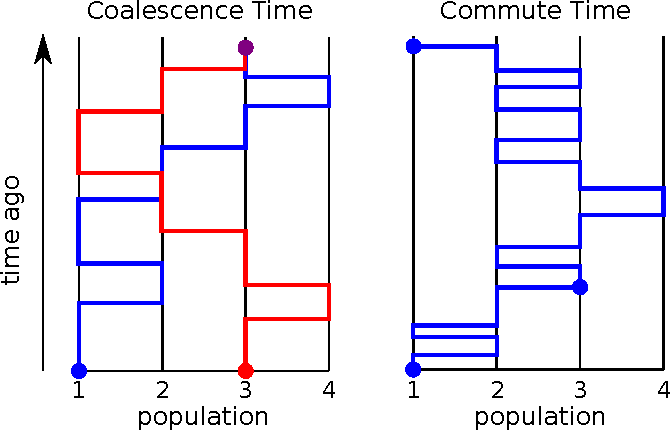
\includegraphics[scale=.5]{figs/conceptn}
    \caption{
    Illustration of the conceptual differences
    betweeen coalescence and commute time between states 1 and 3 
    for a continuous time Markov chain with four linearly connected states. 
    Coalescence time (left) is the time for two independently moving particles to meet and coalesce 
    (it is possible for them to be in the same location without coalescing).
    Commute time is time for a single particle starting in one state to travel to another state 
    and then back to the original state.
    Note how the time axis is scaled to be faster in the figure showing commute time
    than the one for coalescence time in order for them to fit in the same space.
    } \label{fig:concept_coalcom}
\end{figure}


%%%%%%%%%%%%%%%%%%%%%%%%%%%%%%%%%%%%%%%%%%%%
\subsection*{Hitting times of Markov chains}

Now, we explain how to compute the relevant quantities --
mean commute and coalescence times -- from a Markov chain model of lineage movement.
The Markov chain is defined by its \emph{generator matrix}, denoted $G$,
for which $G_{xy}$ gives the jump rate from $x$ to $y$.
This means that if the Markov chain is at location $X_t$ at time $t$,
then for $x \neq y$, the probability the chain jumps from $x$ to $y$ is proportional to $G_{xy}$,
i.e., $\PP{X_{t+\epsilon} = y \given X_t = y} = \epsilon G_{xy} + O(\epsilon^2)$,
and $G_{xx} = - \sum_{y \neq x} G_{xy}$.
We will need to find the \emph{hitting times} of the chain --
i.e., for each pair of states $x$ and $y$, 
the mean time until the chain first hits $y$ after being started at $x$.
We denote this quantity $H_{xy}$.
Throughout, we assume that all hitting times are finite,
which implies the chain is connected and irreducible.
By conditioning on $X_\epsilon$,
one can use the Markov property to show that
\begin{align} \label{eqn:hitting_sum}
    \sum_y G_{xy} H_{yz} = -1 \qquad \text{for} \; x \neq z,
\end{align}
i.e., if $G_{-z}$ is the matrix with the $z^\text{th}$ row and column removed,
and $\bone$ is the vector composed of all ones,
then the $z^\text{th}$ column of $H$, except for $H_{zz}$,
can be computed as $- (G_{-z})^{-1} \bone$.
This, along with $H_{zz} = 0$, allows computation of $H$
from the movement rates $G$.

Suppose instead we are given the hitting times, $H$, and wish to find the movement rates, $G$.
This is not the situation we are in -- we have either commute or coalescence times --
but it is related.
The Random Target Lemma \citep{aldous}
tells us that the stationary distribution of the Markov chain, denoted $\pi$,
can be recovered from the hitting times by solving $\pi = H^{-1} \bone / \bone^T H^{-1} \bone$.
As shown in Appendix \ref{apx::hitting_calcs},
equation \eqref{eqn:hitting_sum} can be rewritten in matrix form as
\begin{align}
    G H = \diag(1/\pi) - \bone \bone^T ,
\end{align}
which implies that $G$ can be computed directly from $H$ as
\begin{align} \label{eqn:G_from_H}
    G = \left( \diag(1/\pi) - \bone \bone^T \right) H^{-1} .
\end{align}
Therefore, $H$ uniquely determines $G$.

% \paragraph{Commute times}
The \emph{commute times} are a symmetrized version of the hitting times
(which need not be symmetric):
\begin{align} \label{eqn:R_from_H}
\text{\bf (commute time)} \qquad
    R_{xy} = H_{xy} + H_{yx},
\end{align}
or $R = H + H^T$.
We use $R$ to refer to the commute time as a reminder that commute times are also effetive resistances,
and to reserve $C$ for the coalescence time.

Although commute times are uniquely determined by movement rates, the reverse is not true.
Commute times only depend on the symmetric part of $H$ --
given an skew-symmetric matrix $Z$ (so that $Z + Z^T = 0$),
any Markov chain that has hitting times given by $H_\epsilon = H + \epsilon Z$ for some $\epsilon$
will have the same commute times.
The resulting hitting times may not be valid --
if we let $G_\epsilon$ be the matrix constructed by applying equation \eqref{eqn:G_from_H} to $H_\epsilon$
(assuming this is invertible),
then it is not guaranteed that the offdiagonal elements of $G_\epsilon$ are all nonnegative, as required.
(It is always true that rows of $G_\epsilon$ sum to zero.)
However, since $G$ and $H$ are continuous functions of each other,
if all offdiagonal elements of $G$ are strictly positive,
then there exists a positive $\epsilon_0$ such that all $G_\epsilon$ for $\epsilon < \epsilon_0$
do define valid Markov chains, all with the same commute times.

% \paragraph{Coalescence times}
The \emph{coalescence times} are defined using \emph{two} copies of the same chain,
as the mean time until coalescence,
if the chains coalesce at rate $\gamma$ when they are in the same place.
Concretely, 
suppose that $X$ and $Y$ are independent Markov chains both moving with movement rates given by $G$,
that coalesce at rate $\gamma_x$ when $X$ and $Y$ are both at $x$.
Then we define $\tau$ to be this coalescence time,
so that 
$\P\{\tau \le t + \epsilon \given \tau > t, \; X_t = Y_t = x\} = \epsilon \gamma_x + O(\epsilon^2)$,
and 
$\P\{\tau \le t + \epsilon \given \tau > t, \; X_t \neq Y_t\} = O(\epsilon^2)$.
Then, the (mean) coalescence time is $C_{xy} = \E[\tau \given X_0 = x, \, Y_0 = y]$.
A similar argument using the Markov property
shows that $C$ satisfies the following equation:
\begin{align}
\text{\bf (coalescence time)} \qquad
    \sum_y \left(G_{xy} C_{yz} + C_{xy} G_{zy}\right)
    &=
    \begin{cases}
        -1                   \quad & \text{if} \; x \neq z, \\
        -1 + \gamma_z C_{zz} \quad & \text{if} \; x = z.
    \end{cases}
\end{align}
Similar recursions are common in the literature,
going back at least to \citet{hill1972effective} (see also \citet{whitlock1997effective}).
In matrix notation, this is
\begin{align} \label{eqn:C_matrix}
    G C + C G^T - \diag(\gamma) \circ C = -\bone \bone^T,
\end{align}
where $\diag(\gamma)$ is the matrix with the vector $\gamma$ on the diagonal and zeros elsewhere,
and $\circ$ is the componentwise product.
In practice, we solve this by working with the product Markov chain $(X_t, Y_t)$,
whose generator matrix is $G \otimes I + I \otimes G$,
where $I$ is the identity matrix and $\otimes$ is the Kronecker product.

Equation \eqref{eqn:C_matrix} is linear in $G$ and $\gamma$,
and so after rearrangement can be solved with standard linear algebra
(and is related to the Sylvester equation \citep{sylvester_eqn}).
However, the solution is again not necessarily unique:
suppose that we have a matrix $Z$ such that $ZC$ is antisymmetric.
Then $(G + Z) C + C (G + Z)^T = GC + CG^T$,
and so a Markov chain with generator matrix $G + Z$ has the same coalescence times
as the original chain.
As before, if all entries of $G$ are nonzero, 
it is always possible to find sufficiently small $Z$
so that $G + Z$ remains the generator of a valid Markov chain,
but this is not guaranteed in general.

\paragraph{Constraints and uniqueness}
We have seen that to find the movement rates of a continuous-time Markov chain
given the coalescence or commute times
we must solve equations \eqref{eqn:C_matrix} or \eqref{eqn:R_from_H} and \eqref{eqn:G_from_H} for $G$,
and that these do not have unique solutions.
The situation is worse when one needs to infer coalescence rates ($\gamma$) as well.
However, usually in applications the locations lie across geographical space,
so that many of the entries of $G$ can be assumed to be zero.
We can get an idea of this by simply counting equations and unknowns.
For concreteness, suppose that the spatial locations
are arranged in a square grid of $n$ locations,
so that each is connected to four others.
(Boundary locations will have fewer, but we omit this detail.)
Since movement rates in each direction can be different,
there are $4n$ free parameters, each corresponding to an offdiagonal entry of $G$.
Coalescence rates provide another $n$ parameters.

Since commute times are symmetric, and $R_{zz} = 0$, 
equation \eqref{eqn:R_from_H} only provides $n (n-1)/2$ informative equations.
This is larger than $4n$, the number of parameters,
for a grid with at least nine nodes (i.e., $3 \times 3$).
The same calculation holds for commute times, 
except that (a) we get an additional $n$ equations from the diagonal entries,
but (b) this is counteracted by the additional $n$ coalescence parameters.

This suggests that although nonuniqueness of solutions may not be a problem in practice,
as long as geography is discretized into sufficiently many locations.
However, another problem appears at finer geographic resolutions:
although solutions may be in principle unique,
the problems become \emph{ill-conditioned} 
in the sense that arbitrarily small variations in the input times
(even numerical instability)
may produce large differences in the inferred rates.
Very roughly speaking, this occurs because as the spatial resolution increases,
the matrix $G$ converges to a second-order elliptic differential operator \citep{pde};
such operators are deformations of the Laplacian \citep{laplacian},
which is well-known to have eigenvalues that decay exponentially \citep{laplacian_eigenvals}.
Information about the landscape contained in higher-order modes
(e.g., finer resolution changes in hitting times)
is then almost obliterated by the small eigenvalues of $G$,
making the inverse problem possible in theory but not in practice.
For more discussion of related problems, see \citet{badtruth,shape_of_a_pop,inverse_prob}.

\paragraph{When are coalescence and commute times equal?}
If in a given biological situation the two times were equal --
i.e., if given $G$ and $\gamma$, there was a $q$ that made $\comdist = C$ --
then inference with either model would be equivalent.
We have already shown that this is not the case in general,
but it turns out that it \emph{is} true
under some restrictive assumptions not uncommonly found in population genetics.
We show in Appendix \ref{sec:com_eq_coal} that
if hitting times are symmetric ($H = H^T$),
then this does occur,
and so the two methods are equivalent for symmetric island models
(where the populations are arranged on a ring 
and migration rates only depend on the distance between them).
Hitting times are not symmetric for a square grid with uniform migration
(the mean time to hit the center from a corner is less than the reverse),
but the square grid is quite close to the torus, which does have symmetric hitting times.


%%%%%%%%%%%%%%%%%%%%%%%%%%%%%%%%%%
\subsection*{The simplest example}

Consider a Markov chain with two states, 
where the rate of movement from state 1 to state 2 is $G_{12}$
and the rate of movement from state 2 to state 1 is $G_{21}$,
so the generator matrix is
\begin{align*}
G = 
    \begin{bmatrix}
        -G_{12}  & G_{12} \\
         G_{21}  & -G_{21}
    \end{bmatrix}.
\end{align*}
Equation \ref{eqn:C_matrix} equates two $2 \times 2$ matrices,
so provides four equations. Only three of these are unique;
simplifying these and using that $C_{12} = C_{21}$, these are:
\begin{align*}
    2 \left(C_{12} - C_{11} \right) G_{12} - C_{11} \gamma_1 &= -1 \\
    \left(C_{11} - C_{12} \right) G_{21} + \left(C_{22} - C_{12}\right) G_{12} &= -1 \\
    2 \left( C_{12} - C_{22} \right) G_{21} - C_{22} \gamma_2 &= -1 .
\end{align*}
Given $C$, we have three equations for the four unknowns, 
$G_{12}$, $G_{21}$, $\gamma_{1}$, and $\gamma_{2}$,
which we can solve symbolically.
The valid solutions to these equations are those with $G_{12}$, $G_{21}$, $\gamma_1$,
and $\gamma_2$ nonnegative.
If $C_{11} \neq C_{12}$, 
we can write the solution with $\gamma_1$ as the free variable:
\begin{align*}
G_{12} &= \frac{1}{2(C_{11} - C_{12})} - \frac{C_{11}}{2(C_{11} - C_{12})}\gamma_1 \\
G_{21} &= \frac{-2(C_{11} - C_{12}) + (C_{12} - C_{22})}{2(C_{11} - C_{12})^2}
	- \frac{C_{11}(C_{12} - C_{22})}{2(C_{11} - C_{12})^2}\gamma_1 \\
\gamma_2 &= \frac{(C_{11} - 2C_{12} + C_{22})^2}{C_{22}(C_{11} - C_{12})^2}
	- \frac{C_{11}(C_{12} - C_{22})^2}{C_{22}(C_{11} - C_{12})^2}\gamma_1.
\end{align*}
This implies that $\gamma_2$ decreases as $\gamma_1$ increases as long as $C_{12} \neq C_{22}$.
This makes sense because
increasing a rate of coalescence cannot make expected coalescence times longer,
so in order to keep coalescence times the same,
if one coalescence rate is increased, another must be decreased.
This also implies that, in order for $\gamma_2$ to be a value other than $0$, 
we must have $C_{11} - 2C_{12} + C_{22} \neq 0$.
In general, if there is a value or range of values of $\gamma_1$
for which the other movement and coalescence parameters are non-negative,
then a solution exists.

\begin{figure}
\centering
         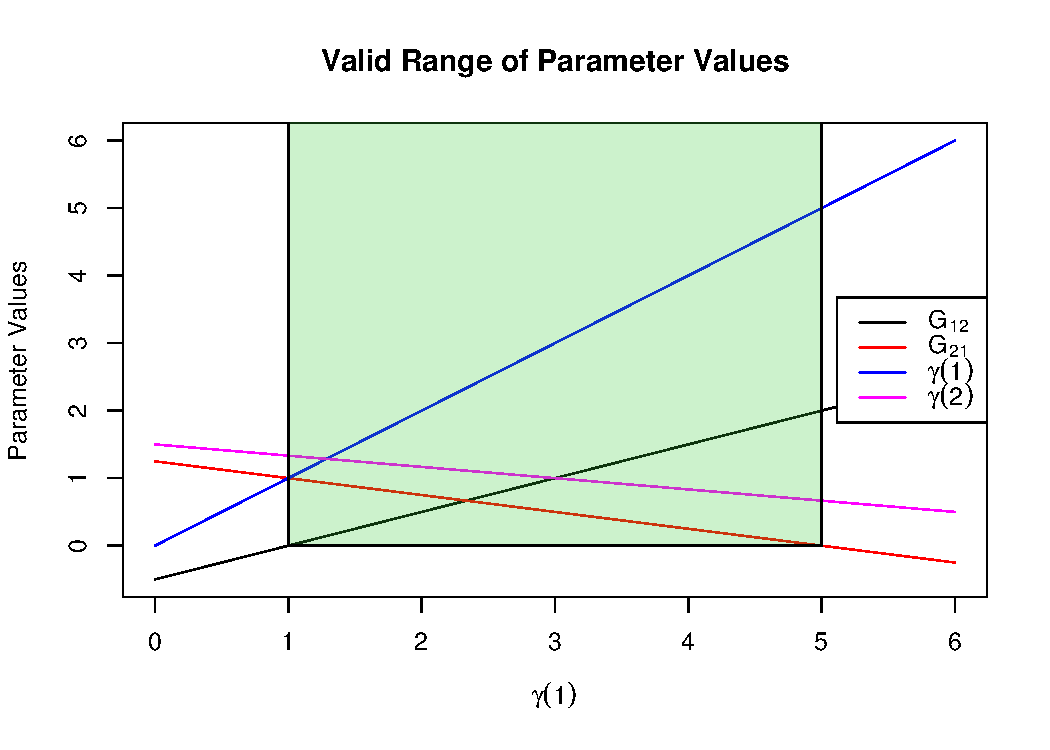
\includegraphics[scale=.7]{figs/valid_range}
    \caption{The green shaded region shows 
        the valid range of the parameter values
        for the two state Markov chain given that
        $C_{11}=1$, $C_{12}=2$, and $C_{22}=1.5$}
    \label{fig:valid_range}
\end{figure}

To produce a comcrete example, suppose that
$C_{11} = 1$, $C_{12} = 2$, and $C_{22} = 1.5$ in arbitrary time units.
The other parameters will be non-negative 
when $1 \leq \gamma_1 \leq 5$,
as shown in in Figure \ref{fig:valid_range}.
Assuming $\gamma_1 = \gamma_2$ produces a unique solution, 
with $\gamma_1 = \gamma_2 = 1.29$ and $G_{12} = 0.14$ and $G_{21} = 0.93$.


%%%%%%%%%%%%%%%%%%%%%%%%%%%%%%%%%%%%
\subsection*{Bayesian inference of movement rates}

Mean coalescence times estimated from real data are subject to a number of sources of noise
(which we discuss in more detail later).
Here, we use
the exact solutions based on linear algebra developed above
to develop a Bayesian inference method that accounts for noise in the data
and estimates uncertainty in the resulting estimates.
To do this, we model genetic distances as equal to coalescence times plus noise:
$D_{ij} = C_{ij} + \epsilon_{ij}$,
where $\epsilon_{ij}$ are independent and Normally distributed
with mean $\mathbf{0}$ and variance $\sigma_\epsilon^2$,
except that $\epsilon_{ij} = \epsilon_{ji}$.
(We imagine that $C_{ij}$ is large compared to $\sigma_{\epsilon}$,
so that resulting values are still positive.)
Using the calculations above, 
given $G$ and $\gamma$ we can compute the corresponding coalescence times
-- which we call $\mathcal{C}(G, \gamma)$ --
so our model is that $D$ has a Gaussian distribution 
with mean $\mathcal{C}(G, \gamma)$.
The maximum likelihood estimate of $G$ could be found directly;
however, this in practice will quite likely contain negative movement rates,
and does not allow us to impose constraints
(such as only allowing a subset of movement rates to be nonzero).

Therefore, we use Bayesian inference,
placing independent exponential priors on the parameters --
the movement rates, $G_{ij}$, that are not constrained to be zero
and the coalescence rates, $\gamma$.
Concretely, suppose that the spatial arrangement of populations is given by a graph,
and only movement rates corresponding to edges in the graph are allowed to be nonzero.
Write $i \sim j$ to mean that $i$ and $j$ are adjacent in the graph,
that there are $m_G$ edges in the graph,
and that each of the $n$ populations has its own coalescence rate.
Then, the resulting log-posterior density is
\begin{align} \label{eq:post}
    \begin{split}
\mathcal{L}(D, G, \gamma) 
    &=
    2 m_G \log(\lambda_G) + n \log(\lambda_\gamma) 
    - \frac{n(n+1)}{2} \log(2 \pi \sigma^2_\epsilon)
	- \sum_{i \sim j} \lambda_G G_{ij}  \\
    &\qquad
    -\sum_{i=1}^n \lambda_{\gamma}\gamma_i
		-\frac{1}{2 \sigma_{\epsilon}^2} \sum_{i \leq j} \left(
            \mathcal{C}_{ij}(G,\gamma) - D_{ij}
        \right)^2 
    \end{split}
\end{align}
Here $1/\lambda_\gamma$ and $1/\lambda_G$ are the prior means of $\gamma_i$ and $G_{ij}$,
respectively.

Inference with commute times is done in exactly the same way,
except that $q$ replaces $\gamma$,
and instead of $\mathcal{C}(G,\gamma)$ we use $\comdistfn(G, q)$,
which is the matrix $\comdist$ computed from $G$ and $q$ by solving equation \eqref{eq:commute_approx}.

It is not required in this approach to have samples from every spatial location,
allowing inference on incompletely sampled spatial discretizations.
To carry out inference in this situation,
we simply use Equation \ref{eq:post},
but only sum over observed entries of $D_{ij}$.

\paragraph{MCMC methods}
To sample from the posterior distribution of equation \eqref{eq:post}, 
we used R \citep{R} 
to implement a standard Metropolis-Hastings algorithm with Gaussian proposals \citep{brooks2011handbook}.
Starting locations were chosen by sampling from the prior distribution.
Before the usual ``burn-in'' phase before sampling for inference begins,
we included a period of ``pre-burn-in'' which used the same MCMC procedure
with a larger $\sigma_\epsilon$, to allow the chain to more quickly converge on the high-posterior
portion of parameter space.
Typically, we ran MCMC for $10^6$ iterations of pre-burn-in 
and $3 \times 10^6$ iterations of burn-in,
followed by $4 \times 10^6$ iterations which were used to estimate posterior distributions,
although for small graphs fewer iterations were necessary.
We used standard methods to assess convergence and mixing.


%%%%%%%%%%%%%%%%%%%%%%%%%%%%%%%%%%%%%%%%
\subsection*{Test cases and simulations}

We compared inference under coalescence and commute time models
using both data ``from the model'' and more realistic simulations.
For the first category, we designed a number of graphs to test particular aspects of inference,
with migration rates specified on each directed edge
(plotted below using igraph \citep{igraph}).
Given the edge weights ($G$) and the coalescence rates ($\gamma$) of a graph,
we produced data by calculating exact coalescence times ($\mathcal{C}(G,\gamma)$),
to whose entries we added independent Gaussian noise while preserving symmetry,
as described above.
Particular parameters and levels of noise are given in the Results.

These simulations are expected to be nearly equivalent to population-based simulations
(either forwards-time or coalescent);
the only difference being that noise terms about the theoretical mean should be somewhat correlated.

\paragraph{Forwards-time simulations}
To produce realistic data, we implemented forwards-time simulations using SLiM v3.0 \citep{haller2017},
with individuals living across continuous, two-dimensional space (sometimes with barriers),
from which we recorded genomic data.
We performed three types of simulation:
uniform migration on a continuous square landscape, 
uniform migration on a rectangular landscape with barriers to migration, 
and biased migration on a square landscape.
Each simulation had $10^4$ diploid, hermaphroditic individuals with nonoverlapping generations.
Mates were selected from nearby individuals using a Gaussian kernel with standard deviation $\sigma_d$,
truncated at $3 \sigma_d$.
Offspring are dispersed away from the mother using the same kernel,
conditioned to lie within the habitable area.
In each simulation, $\sigma_d$ was chosen 
so that there were an average of 0.25 individuals per $\sigma_d^2$ units of area.
In order to prevent excessive population clumpiness \citep{felsensten1975pain}, 
we also model local competition. 
To do this, we use the same truncated Gaussian kernel to define an ``interaction strength''
between each pair of nearby individuals;
then, the fitness of each individual is set to $\exp(-x/40)$, 
where $x$ is the sum of their interaction strengths with other individuals.
This reduces fitness for individuals in denser areas.
Individuals are chosen to reproduce proportional to their fitness.
Clumpiness is similar to what is seen in 
Figure \ref{fig:ind_locs_5x3b_1}.

Individuals have 10 pairs of ``chromosomes'' with $2 \times 10^5$ loci each 
and a recombination rate of $10^{-8}$ per generation per locus.
Mutation rate was $10^{-8}$ per locus for the simulation with uniform migration and no barrier,
and $10^{-7}$ for the remaining simulations.
In all cases, the number of mutations was more than adequate to reliably estimate genetic distance.

To compute genetic distances,
geographic space was partitioned into rectangular regions as depicted below.
within each region, 
individuals are sampled uniformly for ``genotyping'' 
from among those within the middle three quarters of each dimension of rectangle,
as shown for one situation in Figure \ref{fig:ind_locs_5x3b_1}.
This protocol was chosen as a compromise between sampling all individuals 
from near the center of each location,
which could result in a large number of close relatives being sampled, 
leading to an underestimate of the mean genetic distance for individuals in that location
and uniform sampling from the whole area of each grid, 
which may result in many sampled individuals being very close to other grid squares.
Mean genetic distances for each pair of regions is then computed as described above
from genome sequence provided by SLiM.
To estimate uncertainty, we computed the standard error of these mean distances
using the minumum number of individuals in each location.

Before being passed to the MCMC inference method,
we rescaled genetic distances so that the movement rates resulting from the inference
would be approximately of order one.
We did this by multiplying genetic distances by a constant
so that the rescaled mean of the entries of $D$
is equal to the number of locations in the discretization. 



%%%%%%%%%%%%%%%%%%
\section*{Results}
%%%%%%%%%%%%%%%%%%

\plr{transition paragraph}


%%%%%%%%%%%%%%%%%%%%%%%%%%%%%%
\subsection*{Model validation}

We first tested the method using data generated under the model.
To test the methods across a wide range of situations,
we generated random movement rates for 
a large number of $3 \times 2$ rectangular grids:
twenty-five symmetric (i.e., with $G_{ij} = G_{ji}$) and twenty-five asymmetric.
We generated movement parameters
by rounding independent exponential random variables up to the nearest one tenth,
and fixed coalescence rate at 1 for all locations.
We then added independent noise to each matrix entry (preserving symmetry),
and assume that we can estimate the amount of noise reasonably well, 
so used the standard deviation of the noise for $\sigma_\epsilon$ in the likelihood function.
To assess the impact on inference of the number of parameters,
we performed inference both with and without the assumption 
that coalescence rate is the same everywhere.
For $3 \times 2$ graphs, there are 21 equations
and 14 movement parameters,
so that with a global coalescence rate there are 15 unknowns
but with individual coalescence rates there are 20 unknowns,
which is close to nonidentifiable.
(We will not present results from an analogous version of resistance distance inference
that constrains all values of $q$ to be identical
because the true values are not identical, even if all coalescence rates are,
and in practice the method infers true values of $q$ extremely reliably.)
To quantify accuracy across these random graphs in different situations,
we computed, for each model fit on a particular random graph,
the absolute difference between the posterior median of each movement parameter
and the true value.
We then averaged these across movement parameters to produce a measure of accuracy for that model fit,
reported below as ``mean absolute error''.


\paragraph{Varying noise}
Unsurprisingly, coalescence time inference became less accurate as the amount of noise increased.
As we varied the standard deviation of the noise
from 1/1000 to 1/50 of the mean value of $C$ for that grid,
the mean absolute error 
for coalescence time inference with a single coalescence rate
increased from around 0.05 to 0.4.
Posterior interquartile ranges increased proportionally.
(although there was substantial variation in accuracy between replicates;
see Figures \ref{fig:mult_noise} and \ref{fig:mult_noise_iqr}).
Increasing the number of parameters by allowing multiple coalescence rates
made the inference problem even harder --
mean absolute errors no longer depended strongly on the amount of noise added,
and hovered around 0.4.

More surprisingly, the performance of commute time inference did not depend on the amount of noise --
mean absolute error was around 0.6 across all levels of noise,
both with and without more than one parameter for local diversity
(see Figure \ref{fig:mult_noise}).
Although symmetry did not affect coalescence time inference,
commute time inference did substantially worse on asymmetric graphs,
showing median absolute errors of around 0.8.

\paragraph{Varying coalescence rates}
Lower coalescence rates mean that lineages wander about the landscape for longer
before they coalesce, 
thus greatly reducing the geographic information we get from coalescence times.
Indeed, coalescence rates had a strong effect on feasability of the inference problem
(shown in Figures \ref{fig:mult_gam} and \ref{fig:mult_gam_iqr}):
lowering the coalescence rate from 10 to 0.1
(always adding noise with standard deviation 1/200th of the mean value)
increased mean absolute error of coalescence time inference from around 0.05 to 0.5.
Again, allowing multiple coalescence rates
or using commute time inference were highly inaccurate in all cases,
with mean absolute errors of above 0.5.


%%%%%%%%%%%%%%%%%%%%%%%%%%%%%%%%%%%%%%%%%%%%%%%%
\subsection*{Identifying a barrier to gene flow}
\label{sec:5x3b}


We then test the method's ability to locate barriers to migration
on the $5 \times 3$ grid with asymmetric gene flow shown in Figure \ref{fig:5x3b_grid}. 
Each nonzero movement rate is determined randomly as before.
Coalescence rates are set to 1 everywhere.
Figure \ref{fig:5x3b_post_coalvcom} shows posterior distributions of the movement rates
for both coalescence time and resistance distance inference
on this graph, with noise standard deviation equal to
1/1000 of the mean coalescence time (left)
and 1/100 of the mean coalescence time (right).
Although increased noise in the data increased uncertainty in the estimated values,
coalescence time inference correctly inferred not only the location of the barrier
but also the migration rates along all other edges within a reasonable margin of error.
Commute time inference also identified the barrier,
but was much less accurate for the other values.
We also explored making the problem harder,
by first (a) dropping rows and columns from the data corresponding to populations 2, 5, 7, and 15;
and then (b) allowing a separate coalescence rate for each location,
in both cases using a noise level of 1/100.
The resulting posterior distributions are shown in Figure \ref{fig:5x3boxplots_mult_gam},
and show substantially increased error,
but only in movement rates to the removed locations.
As before, uncertainty was increased when multiple coalescence rates were allowed,
but not as strongly as before, likely because the problem is less close to being underconstrained,
having 105 equations and 59 unknowns.


\begin{figure}
\centering
     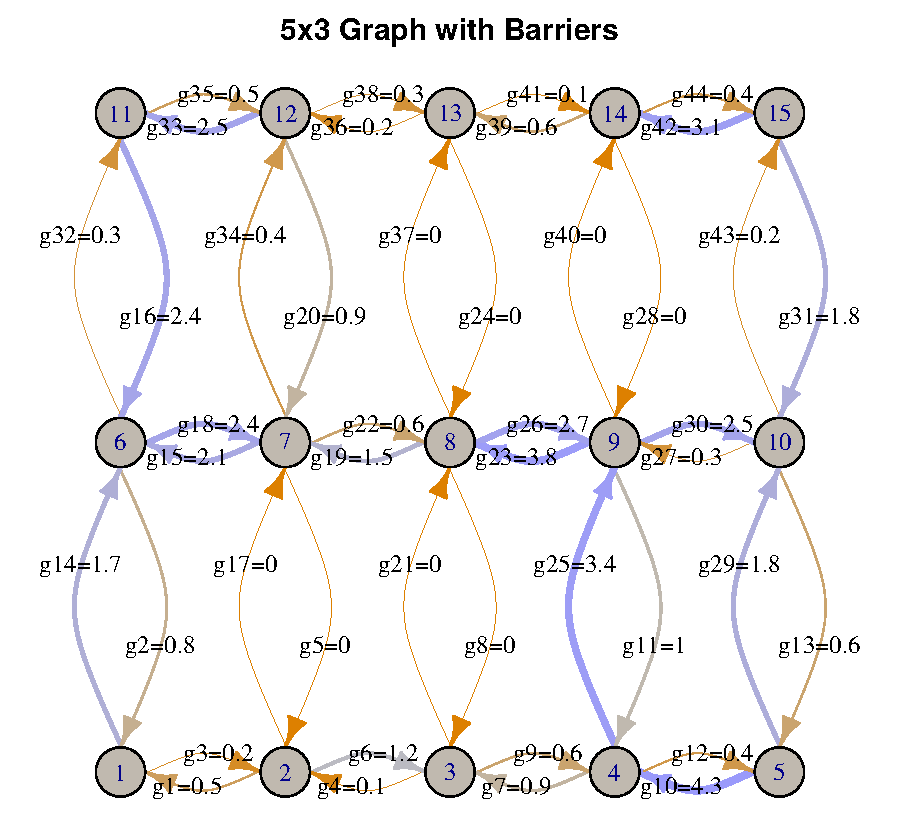
\includegraphics[scale=.6]{figs/5x3b_grid}
    \caption{Plot of the grid structure 
    for the 5 $\times$ 3 grid with two barriers:
    movement rates between $\{2,3\}$ and $\{7,8\}$ are zero,
    as are those between $\{8,9\}$ and $\{13,14\}$.
    Values for the non-zero movement rates 
    were chosen by rounding independent draws of an exponential random variable with mean 1 
    up to the nearest tenth.
    } \label{fig:5x3b_grid}
\end{figure}

\begin{figure}
\centering
     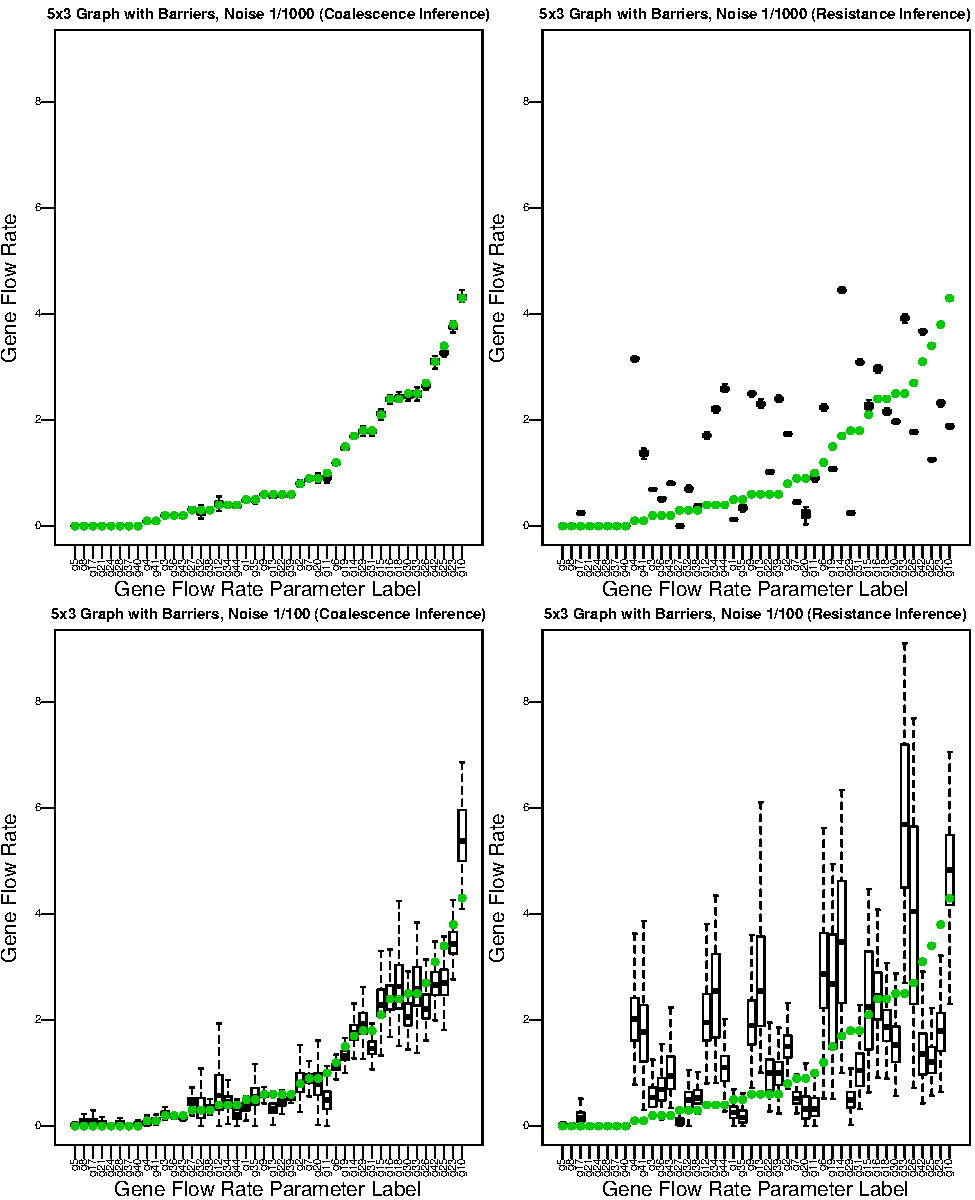
\includegraphics[scale=1]{figs/5x3b_post_coalvcom}
    \caption{Posterior distributions for values of $g$ 
    for the 5 $\times$ 3 graph with barriers 
    with two different noise levels with both coalescence time and resistance distance inference.
    See Figure \ref{fig:5x3b_grid} to see movement parameter locations.
    %\plr{TODO: replace bottom two panels with same thing for commute time (eg figs/5x3b100\_com.pdf);
    %     put this figure in the supplement}
}
    \label{fig:5x3b_post_coalvcom}
\end{figure}


%%%%%%%%%%%%%%%%%%%%%%%%%%%%%%
\subsection*{Biased migration}
\label{sec:biased_migration}

Both matrices of coalescence and commute times, $C$ and $R$, are symmetric,
but they do not deal with asymmetric (biased) migration in the same way.
Since commute time to $i$ requires paths both to and from $i$,
but coalescence time to $i$ only reaquires lineages to leave $i$,
if, for instance, there is a low rate of migration back into $i$,
then commute times to $i$ could be quite long even while coalescence times are not.
For instance, suppose there are three populations arranged in a line,
and lineages currently in the outer populations are much more likely to come from the central population
than the other way around.
Since lineages quickly move to the center and coalesce regardless of starting position,
coalescence time (and genetic diversity) will be relatively low between all individuals.
Commute time between the two outer locations, on the other hand,
will be much longer than other comparisons, since it requires a lineage to leave the center.

In order to investigate this general situation,
we tested both methods on four different $4 \times 4$ graphs (shown in Figure \ref{fig:4x4_grids}):
\emph{uniform}, where all movement rates are 1.0;
\emph{symmetric}, where movement rates are symmetric and randomly generated as before;
\emph{asymmetric}, where all movement rates are random;
and \emph{biased}, where movement rates down or to the left are equal to 2.0,
and movement rates up or to the right are 0.5.
For inference, we added noise with standard deviation $1/500^\text{th}$ of the mean value.

Differences between true mean coalescence times ($C$) and mean commute times ($\comdist$) 
are shown in Figure \ref{fig:RvsC}:
they are fairly small in the uniform and symmetric cases, moderate in the asymmetric case, 
and extreme in the biased asymmetric case.
This difference suggests that commute time inference may be strongly misled 
in the asymmetric and biased situations,
but it still could be the case that the movement rates that give the best fit of commute time
to coalescence time data could be close to the actual rates use to generate the data.

Nonetheless, 
coalescence time inference was substantially more accurate in all cases.
Posterior distributions of movement parameters are shown in Figure \ref{fig:4x4box},
produced by applying both inference methods
after adding noise with standard deviation of 1/200 the mean value of $C$.
The mean absolute errors for coalescence time inference are 0.12 or less in all cases.
Commute time inference obtains roughly uniform migration rates
(although varying by a factor of 2) in the uniform case;
and migration rates noisily correlated with the truth in the symmetric graph.
However, commute time inferences for the asymmetric and biased graphs are only weakly correlated, 
if at all, to the truth.
Commute times also drastically overestimate movement rates for the biased case,
as we would expect based on the differences discussed above.


\begin{figure}
\centering
     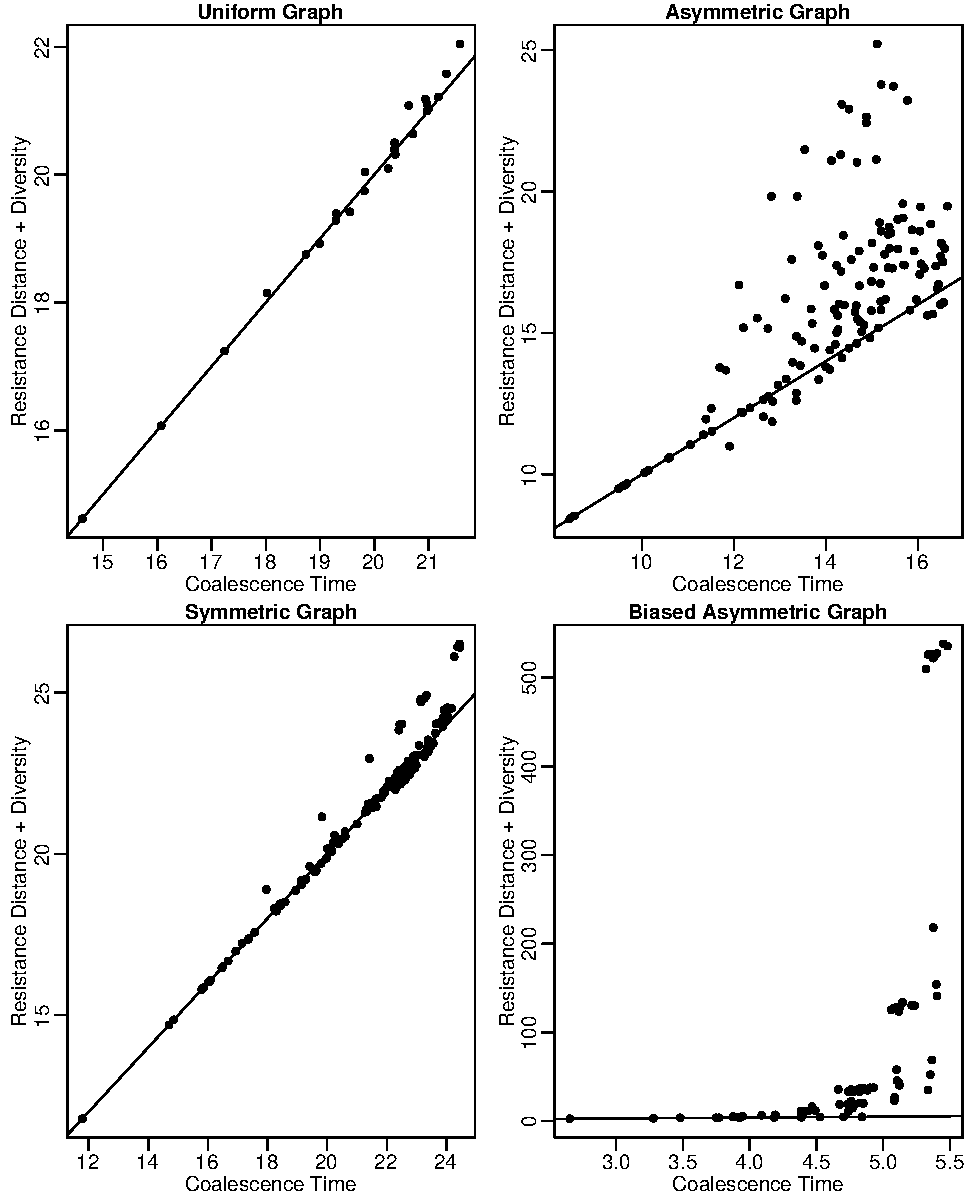
\includegraphics[scale=1]{figs/RvsC}
    \caption{Plots of the true values of $\comdist$ vs $C$ 
    for the uniform graph, symmetric graph, the asymmetric graph,
    and the biased asymmetric graph, 
    shown with the $y=x$ line.
    %\plr{TODO: make this a 2x2 grid instead of 4x1}
    See Figure \ref{fig:4x4_grids} to see overall graph structure.}
    \label{fig:RvsC}
\end{figure}

\begin{figure}
\centering
     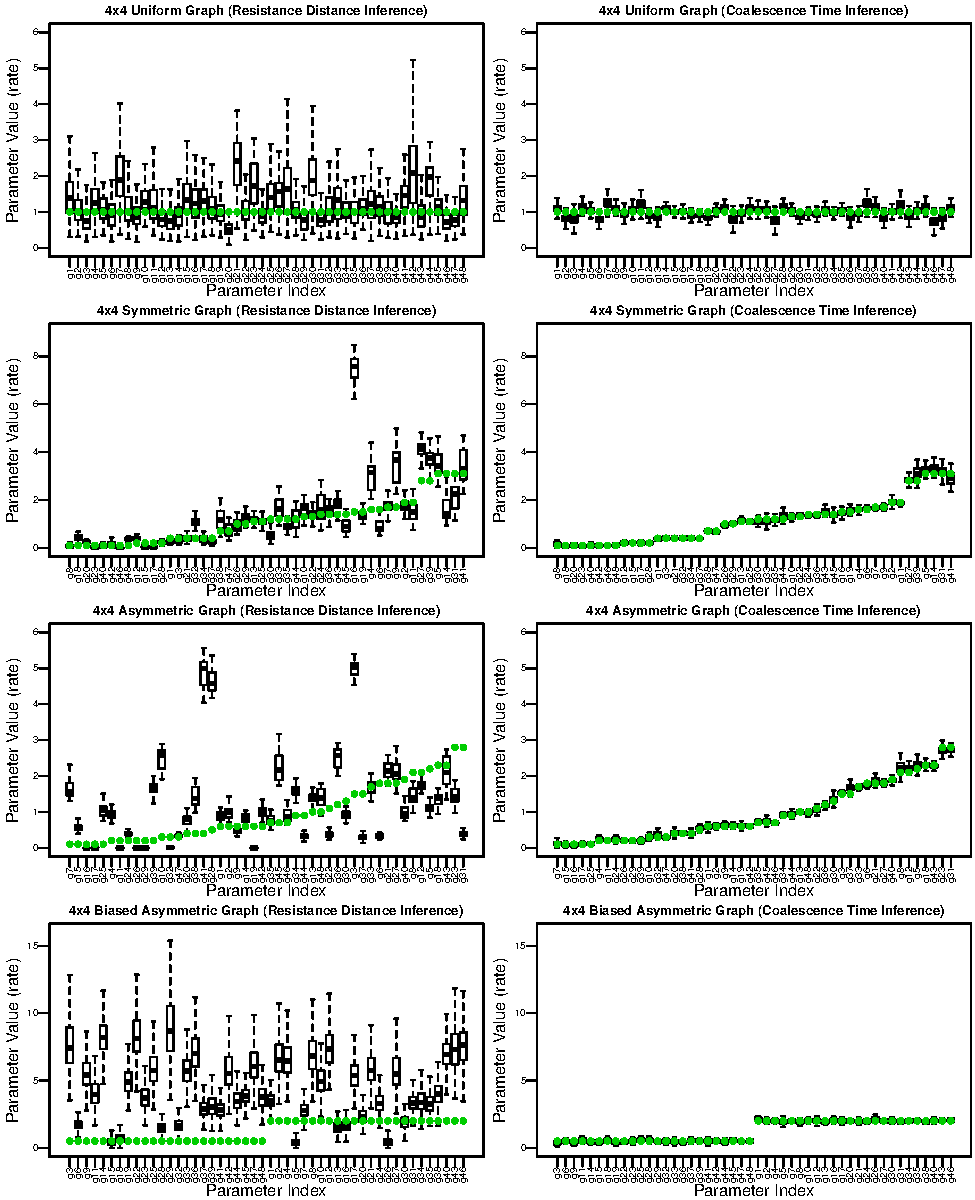
\includegraphics[scale=1]{figs/4x4boxplots_paper}
    \caption{Boxplots of the posterior distributions for $g$ for commute time and coalescence time
    based inference for the uniform graph, symmetric graph, 
    the asymmetric graph, and the biased symmetric graph.
    See Figure \ref{fig:4x4_grids} to see movement parameter locations.}
    \label{fig:4x4box}
\end{figure}


%%%%%%%%%%%%%%%%%%%%%%%%%%%%%%%%%%%%%%%%%%%
\subsection*{Continuous geographical space}

The data we have used thus far are produced ``under the model'',
and should provide an accurate depiction of our method applied to discrete, randomly mating populations
whose connections by migration are known.
However, this is nearly always a rough approximation to reality,
in which organisms are distributed across continuous geography,
and ``populations'' are constructed by necessity, often driven by sampling locations.

\paragraph{Process noise}
The mean coalescence times of lineages that we compute analytically
are exact for large, randomly mating populations,
but the word ``mean'' indicates an average across several levels of randomness:
and observed, empirical mean estimated using a sample of genotyeps
will differ slightly depending on both the individuals sampled (``sampling noise'')
and the stochasticity of the population history itself (``process noise'').
For more discussion of this latter contribution in other contexts, see
\citet{waples}, \citet{wakeley}, or \citet{ralph_empirical}.
In populations living across continuous geography,
both sources of noise can be substantially larger due to randomness in spatial locations.
A hint of this is visible in Figure \ref{fig:ind_locs_5x3b_1},
where we see that the distribution of individuals across the landscape
is fairly patchy.
This might make inference using a discretization of continuous space considerably more difficult.

To quantify the relative contributions of the different sources of noise,
we coompared mean genetic distances, calculated in the same way,
between nonoverlapping sets of samples from the same simulation,
and between different simulations.
These simulations were done using SLiM as described in the Methods
on a square, $4 \times 4$ landscape with no barriers.
We found that process noise was much larger than sampling noise --
as shown in Figure \ref{fig:h_val_comp},
discrepancies between simulations are about five times that seen
between different samples from the same simulation.
An implication of this is that uncertainties in genetic distance
estimated from the data will be (possibly large) underestimates,
a fact also pointed out for effective population size by \citet{waples}.


\begin{figure}
\centering
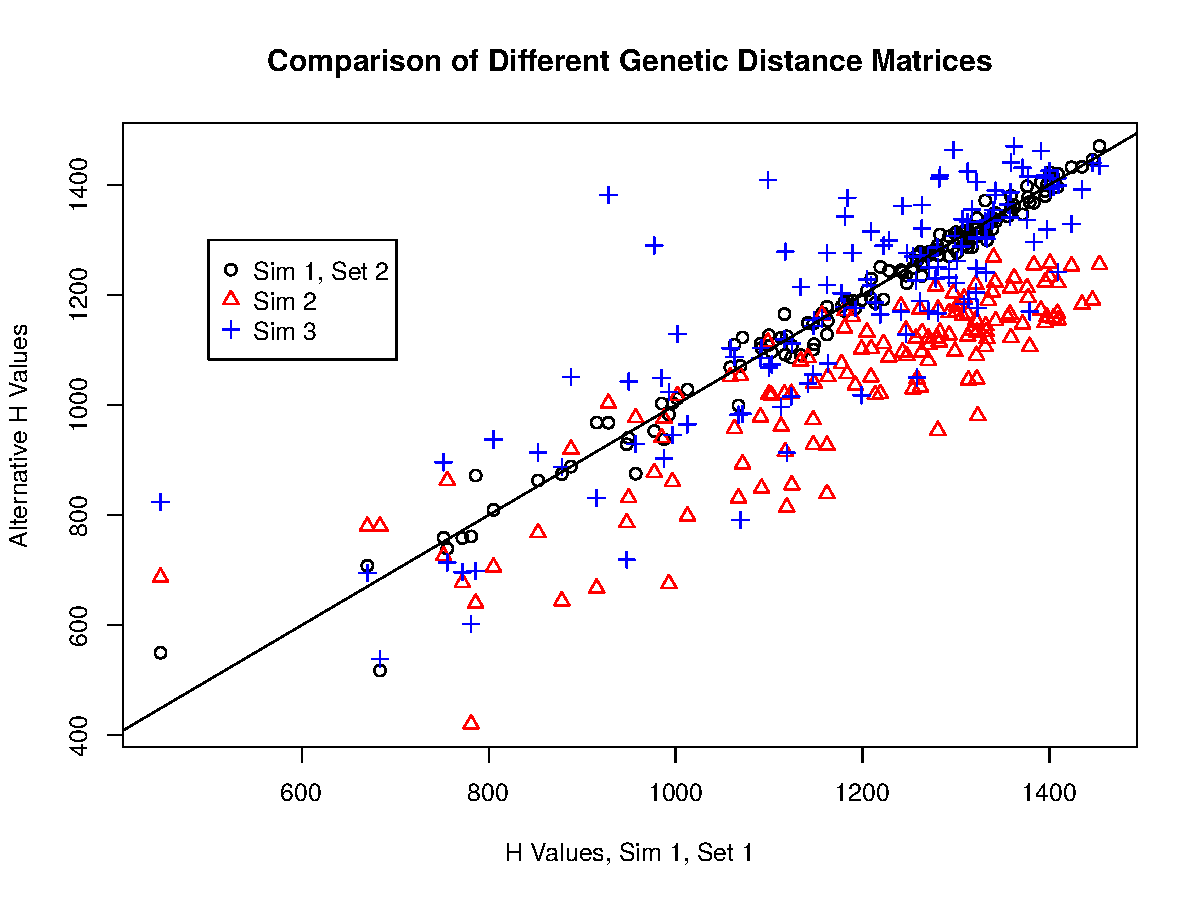
\includegraphics[scale=.8]{figs/h_val_comp}
\caption{
    Comparison of the values of the genetic distance matrix $C$
    for a $4 \times 4$ discretization of a square landscape with uniform migration
    calculated from various situations.
    All values are plotted against the corresponding values from the $C$ matrix
    calculated using the first set of individuals from the first simulation,
    along with the $y=x$ line.
    Black circles are from a second (non-overlapping) set of individuals from the first simulation,
    red triangles are from the second simulation, 
    and blue plusses are for the third simulation.
    Mean absolute value relative differences between the new values of $C$ for each situation
    and the original values from the first set of individuals from the first simulation are
    1.8\% for the second set of indivuals from the first simulation,
    13.2\% for the second simulation, 
    and 7.3\% for the third simulation.
    } \label{fig:h_val_comp}
\end{figure}

\paragraph{Identifying a barrier}
We now revisit the earlier situation where a landscape has locations that are barriers to gene flow,
as in Section \ref{sec:5x3b}.
The landscape is designed to be a continuous version of this situation.
Since the distribution of offspring locations is truncated at three standard deviations
away from the mother, a sufficiently thick uninhabitable area can completely stop migration
directly across it.
As in \ref{sec:5x3b}, though, the landscape is still relatively well connected.
The layout of the landscape can be seen in Figure \ref{fig:ind_locs_5x3b_1},
with the red bars being the uninhabitable regions that serve as barriers to migration.
Unlike the case of a square landscape with no barriers, 
there is not a natual way to discretize it more coarsely 
with grid squares of equal size and shape,
so a $5 \times 3$ grid will be the only discretization used in this section.
We calculate mean genetic distances using 50 individuals 
from each grid location,
here giving us a total of 750 individuals.


\begin{figure}
\centering
     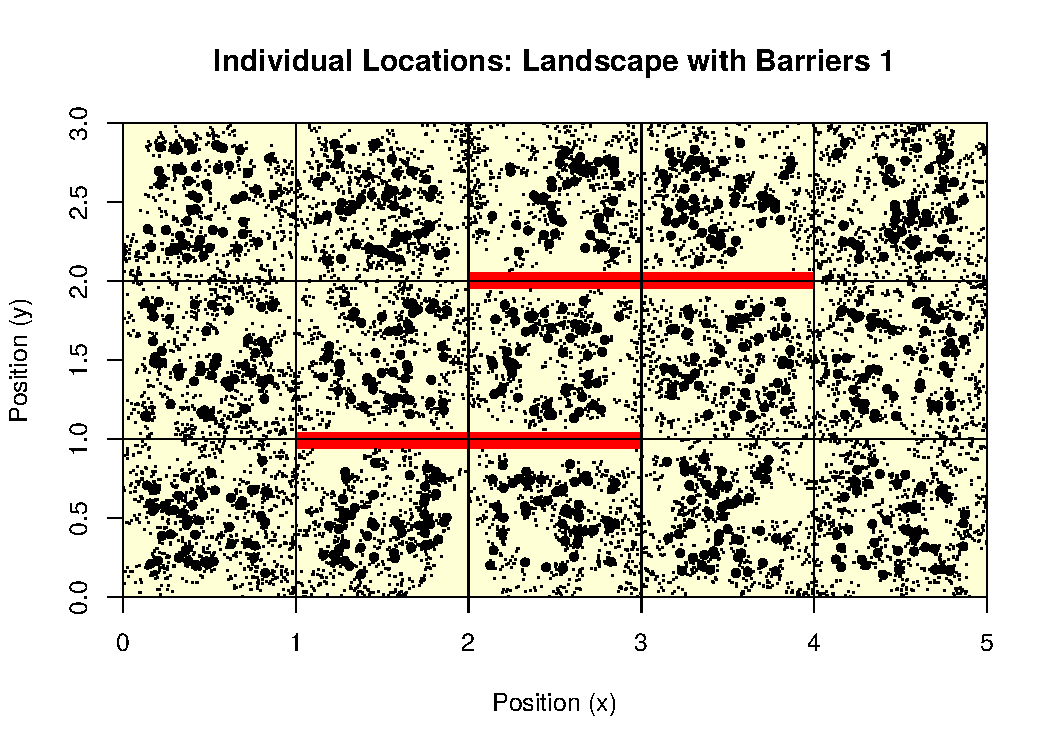
\includegraphics[scale=.8]{figs/ind_locs_5x3b_1}
    \caption{Locations of all and selected individuals on the $5 \times 3$ landscape with barriers
    in the first replicate.
    Locations of individuals used to compute the mean genetic distance matrix are shown in bold points
    whereas the locations of other individuals are shown in smaller points.
    The red bars show the locations of uninhabitable regions of the landscape.
    They are sufficiently thick so that no migration can occur directly across them.}
    \label{fig:ind_locs_5x3b_1}
\end{figure}

\begin{figure}
\centering
     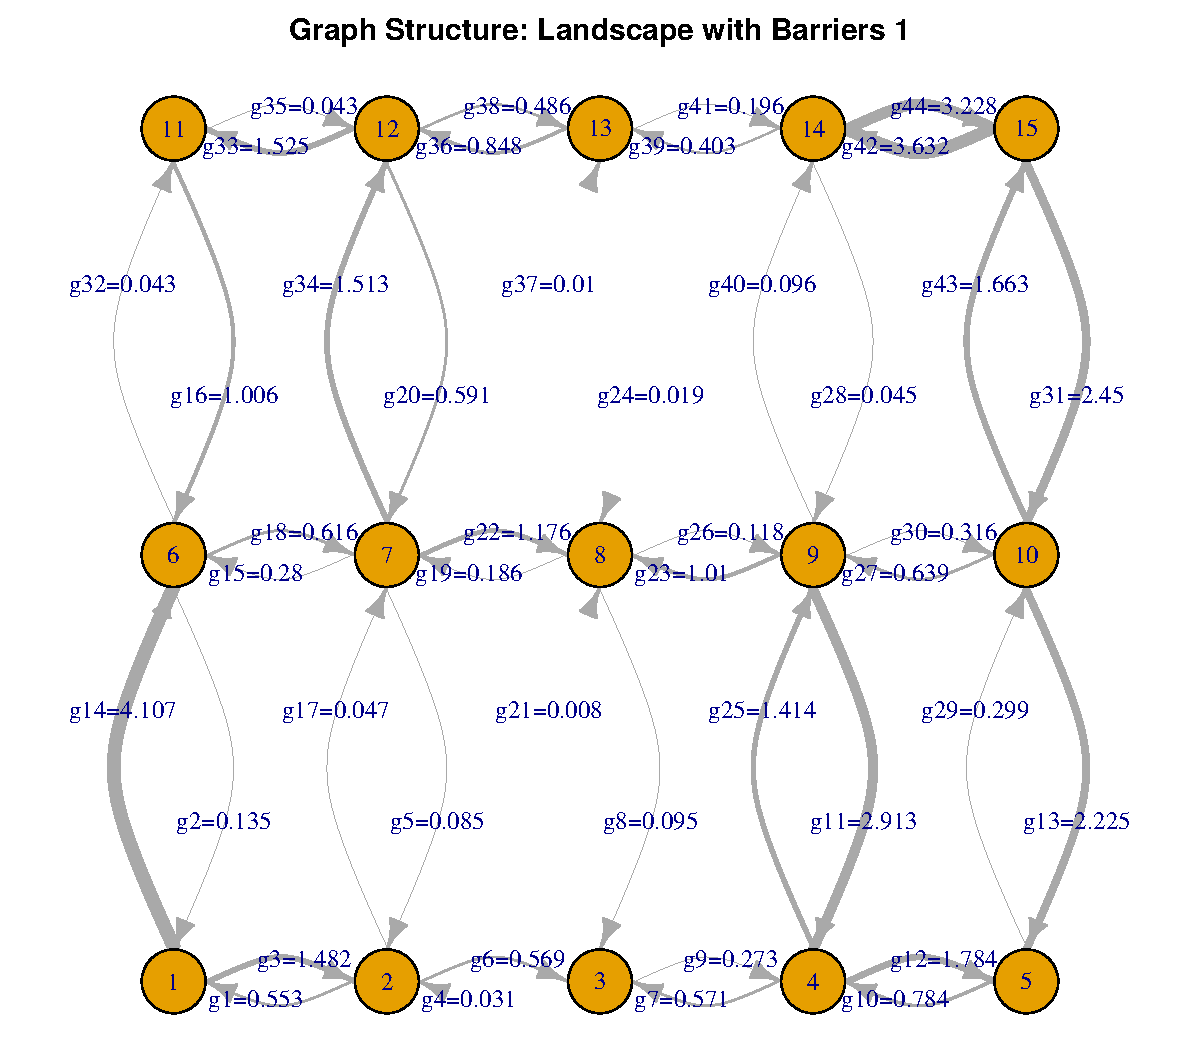
\includegraphics[height=0.3\textheight]{figs/grid_5x3b_1}
     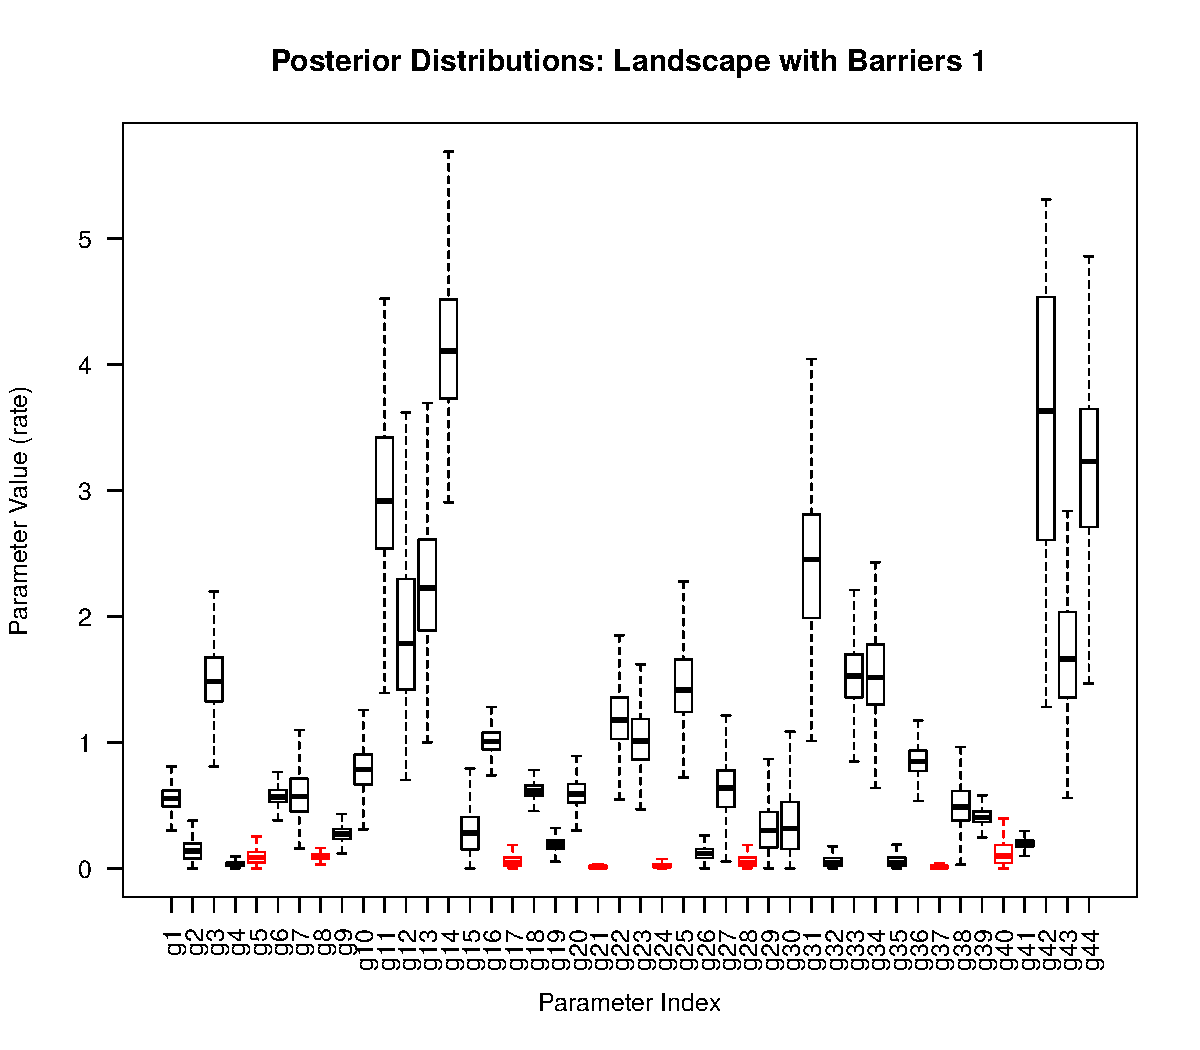
\includegraphics[height=0.3\textheight]{figs/post_dists_5x3b_1_new}
    \caption{
    \textbf{(top)}
    Posterior medians of movement rates for a replicate of the continuous landscape
    with barriers depicted in Figure \ref{fig:ind_locs_5x3b_1}.
    \textbf{(bottom)}
    Boxplots of the same posterior distributions,
    colored red for gene flow rates of edges that cross the barrier.
    } \label{fig:post_dists_5x3b_1}
\end{figure}

The gene flow rates across the barriers are reliably estimated to be very small
%(\emph{maybe reference all 6 supplemental figures here?}),
but there is considerable variation in the other values.
Note, however, that this analysis requires that we guess a reasonable place
to put the divisions between the locations.
For instance, we may wonder whether a river or other geographical feature
restricts gene flow.
We would then discretize the landscape such that individuals on opposite sides of the 
potential obstruction are in separate grid spaces.


\paragraph{Continuous Landscape with Biased Migration}
The third situation that we will discuss is where migration is biased.
We will be using a square landscape as in the first case, 
but the offspring locations of offspring are not centered around the parent.
Instead, the mean of the distribution of the locations
is one tenth of a standand deviation (or 0.05\% of the edge length of the landscape) 
up and to the right of their parent's location.
This results in reverse time gene flow down and to the left 
as in the biased asymmetric graph in Section \ref{sec:biased_migration}.
In terms of population genetics, 
this is very similar to the case where a population is expanding into new territory 
since in both cases, 
offspring tend to be further from the edge of the expansion than their parents.
The difference is that, in our case, 
the population is constrained to be a bounded distance 
away from the edge of the ``expansion''.
In both situations, individuals at the edge may have disproportionately more offspring,
leading to low genetic diversity and strong drift.
This results in substantially more noise in the isolation by distance plots 
as seen in Figure \ref{fig:ibd_comp}. 
The horizontal lines in that figure are likely from comparing genomes of individuals from
two families that have recently increased in size and geographical spread, 
resulting in many pairs of genomes with similar genetic distance 
but varying geographic distance.

As in Section \ref{sec:slim_unif}, we discretize the landscape into
both a $2 \times 2$ grid and a $4 \times 4$ grid for inference.
Looking at the medians of the inferred posteriors of the gene flow rates in the $2 \times 2$ case
(Figure \ref{fig:2x2grid_asb}),
it is immediately clear how strong the bias 
against reverse time gene flow out of the lower left corner is.
That is, hardly any individuals in the lower left area have ancestors
from other regions of the landscape.
This is to be expected as even though the single generation migration bias is small,
having a descendant in a location against the bias after a large number of generations
becomes less and less likely as the number of generations increases.
In the $4 \times 4$ discretization, 
the bottom left also shows very strongly biased gene flow (Figure \ref{fig:grid_bias_4x4_1}).
Most (but not all) of the other pairs also show bias in the expected direction.
Boxplots of the posterior distributions are shown in Figure \ref{fig:post_dists_bias_4x4_1}.
%\emph{maybe talk about/cite some biased random walk stuff here?}

%\emph{talk about some kind of log ratio test for the 4x4 case?}

\begin{figure}
\centering
 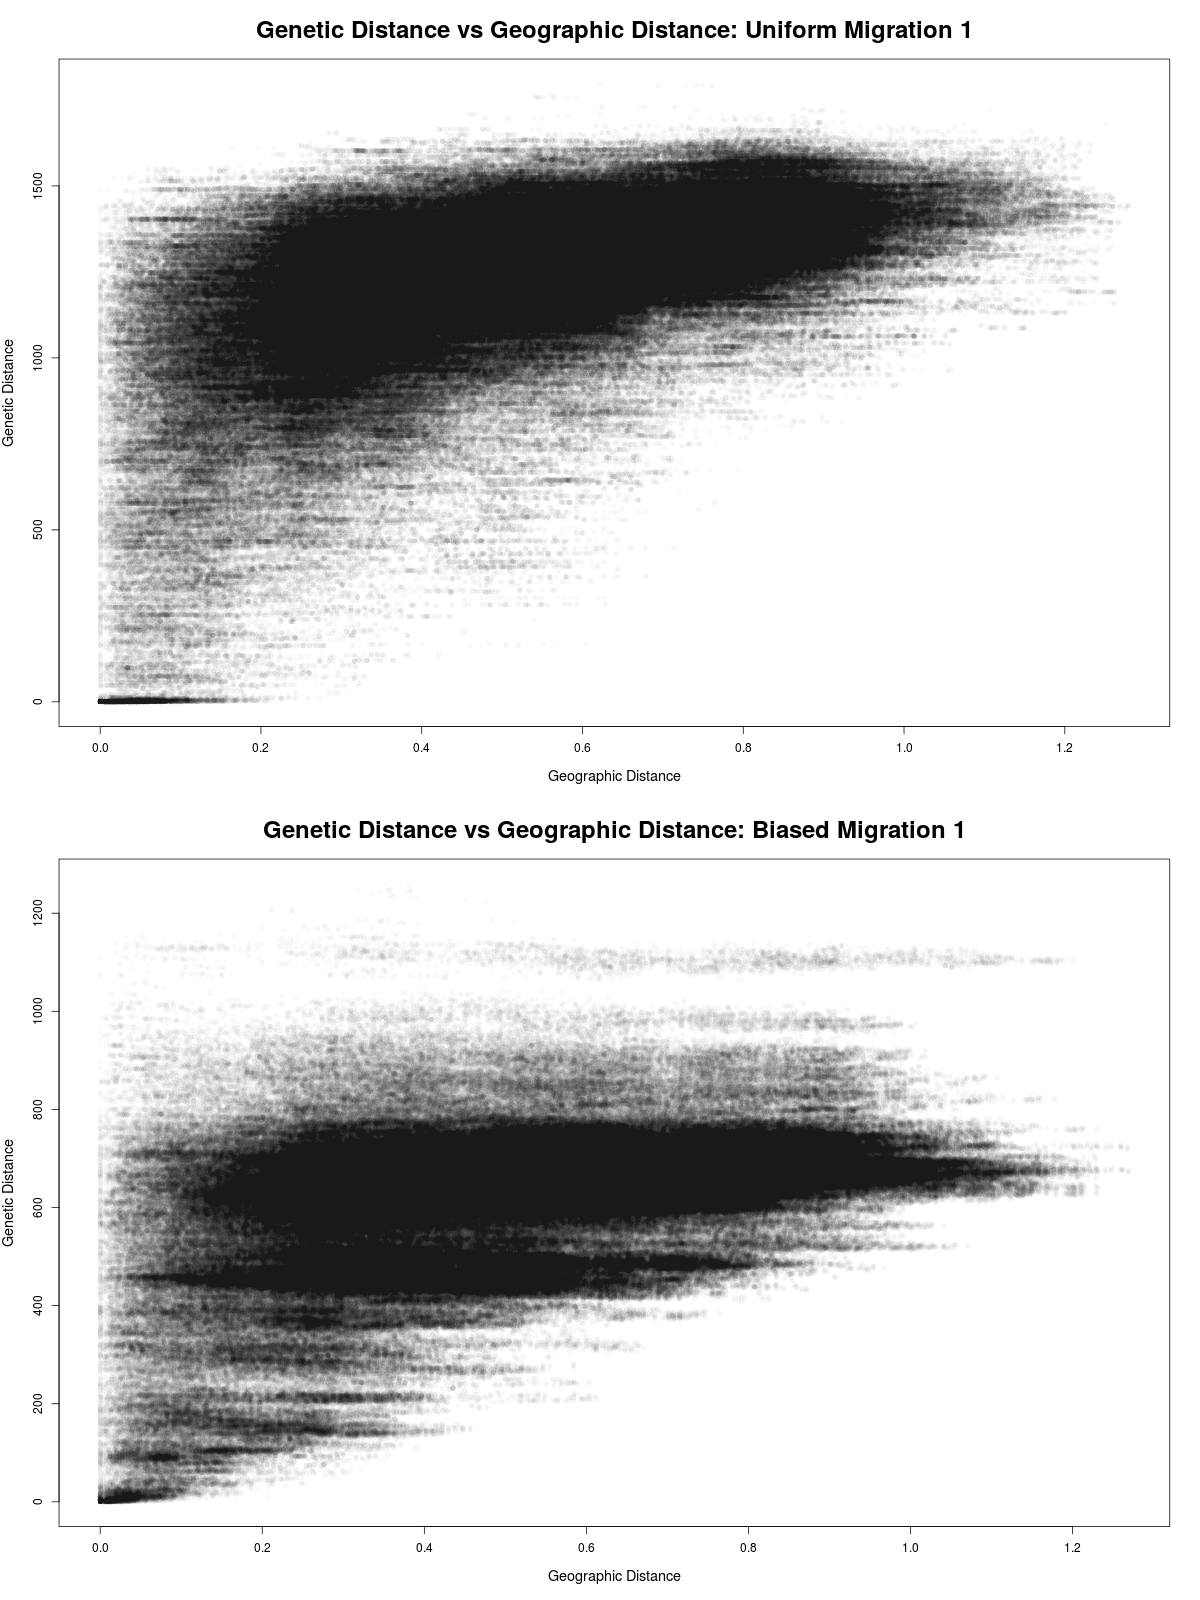
\includegraphics[scale=.35]{figs/ibd_comp}
\caption{Comparison of the isolation by distance plots for the square landscape with uniform migration
and the square landscape with biased migration.
Faster coalescence in the biased migration case results in more noticeable horizontal lines,
indicative of families that recently increased in size and geographical spread.}
\label{fig:ibd_comp}
\end{figure}


\begin{figure}
\centering
 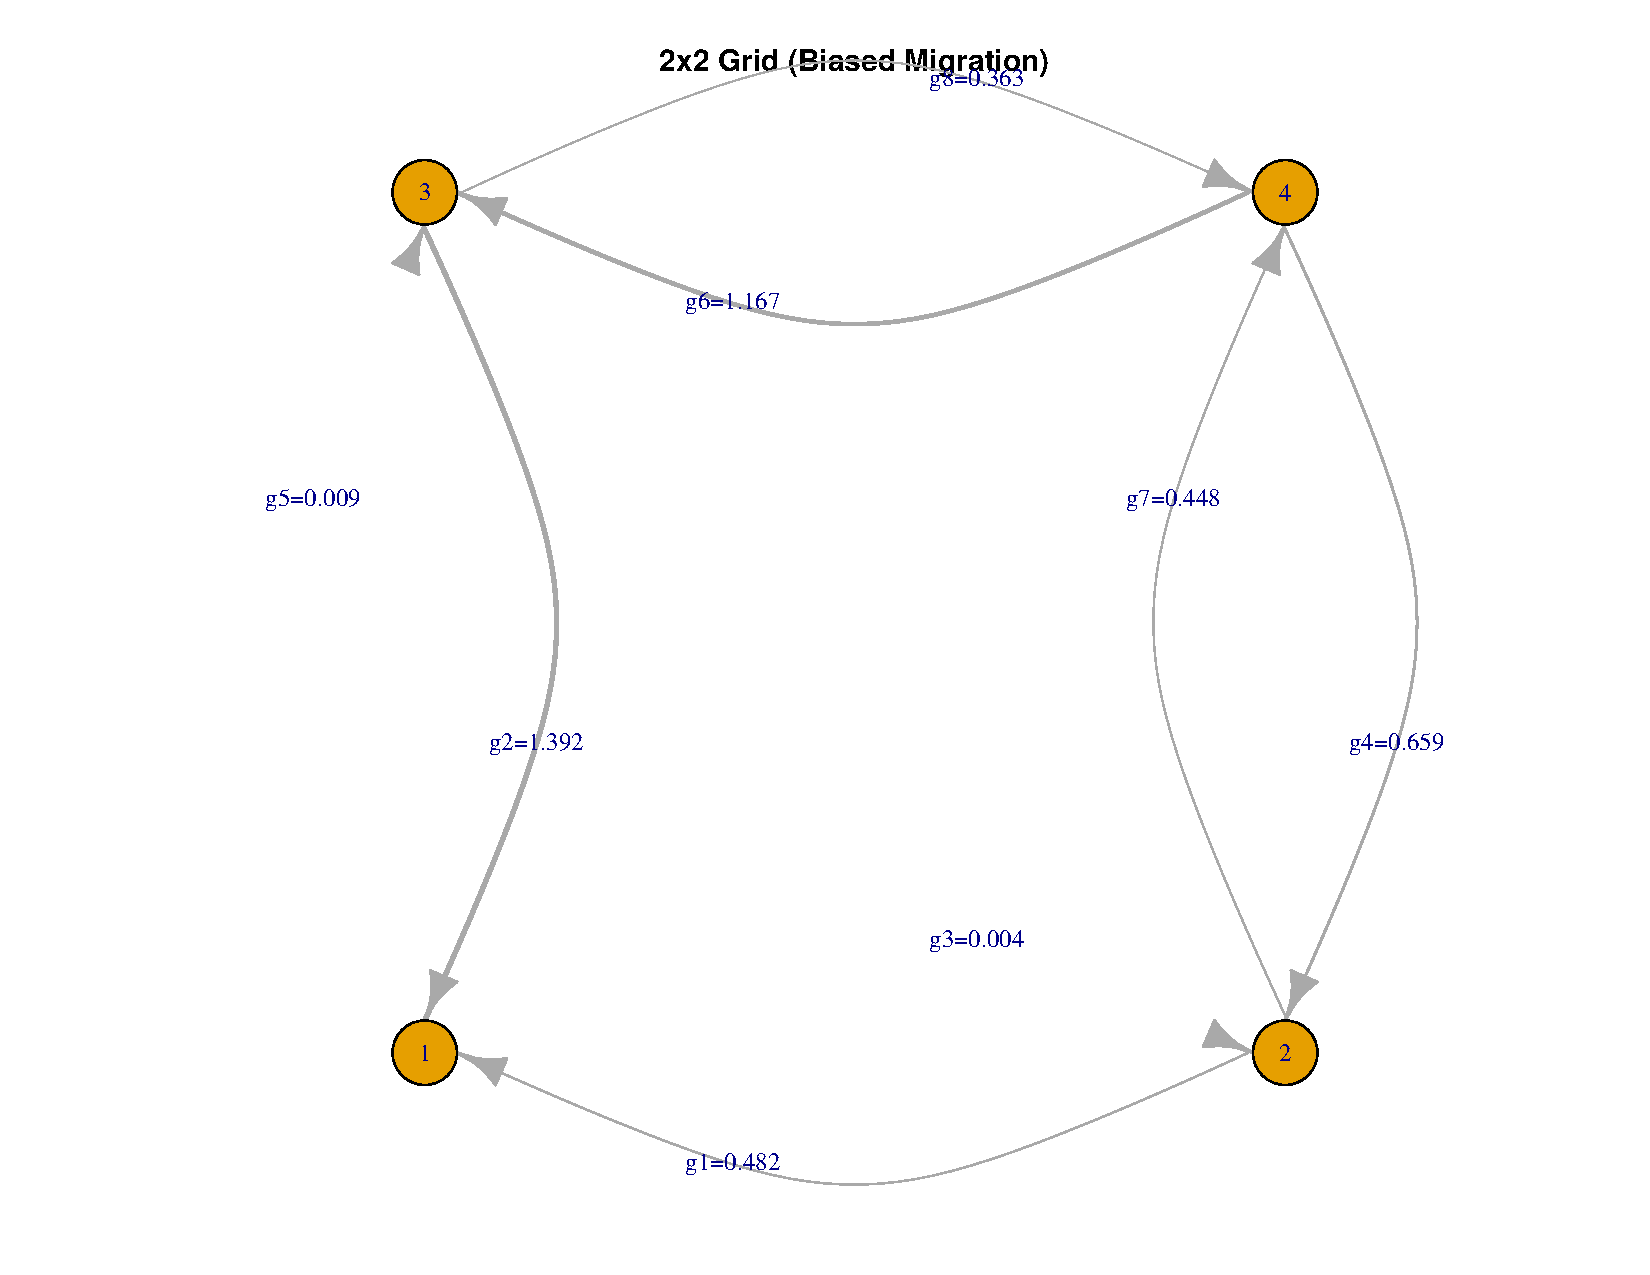
\includegraphics[scale=.5]{figs/2x2grid_asb}
\caption{Medians of the posterior distributions of the inferred values of $g$ 
for the first replicate of the $2 \times 2$ discretization of the square landscape with biased migration.
The reverse time gene flow rates out of the bottom left section are very small,
indicating that very few individuals living in the bottom left of the landscape
have ancestors from other regions of the habitat,
consistent with migration biased up and to the right.}
\label{fig:2x2grid_asb}
\end{figure}

\begin{figure}
\centering
 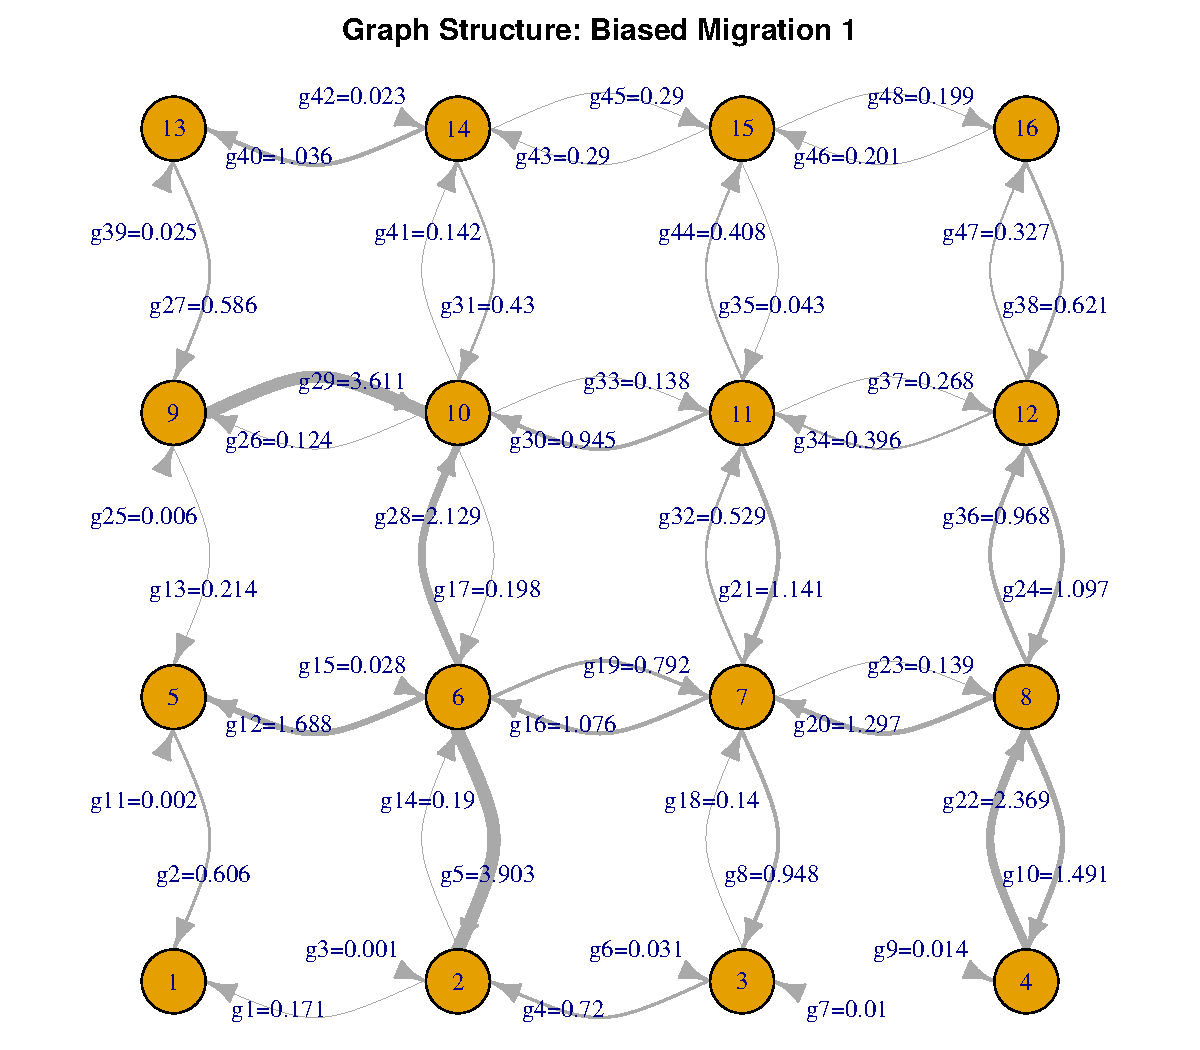
\includegraphics[scale=.8]{figs/grid_bias_4x4_1}
\caption{Medians of the posterior distributions of the inferred values of $g$ 
for the first replicate of the $4 \times 4$ discretization of the square landscape with biased migration.
As in the $2 \times 2$ case, 
the reverse time gene flow rates out of the bottom left section are very small,
indicating that very few individuals living in that area of the landscape
have ancestors from other regions of the graph.
Most, but not all of the other gene flow rates are biased 
in the direction we would expect.}
\label{fig:grid_bias_4x4_1}
\end{figure}

\begin{figure}
\centering
 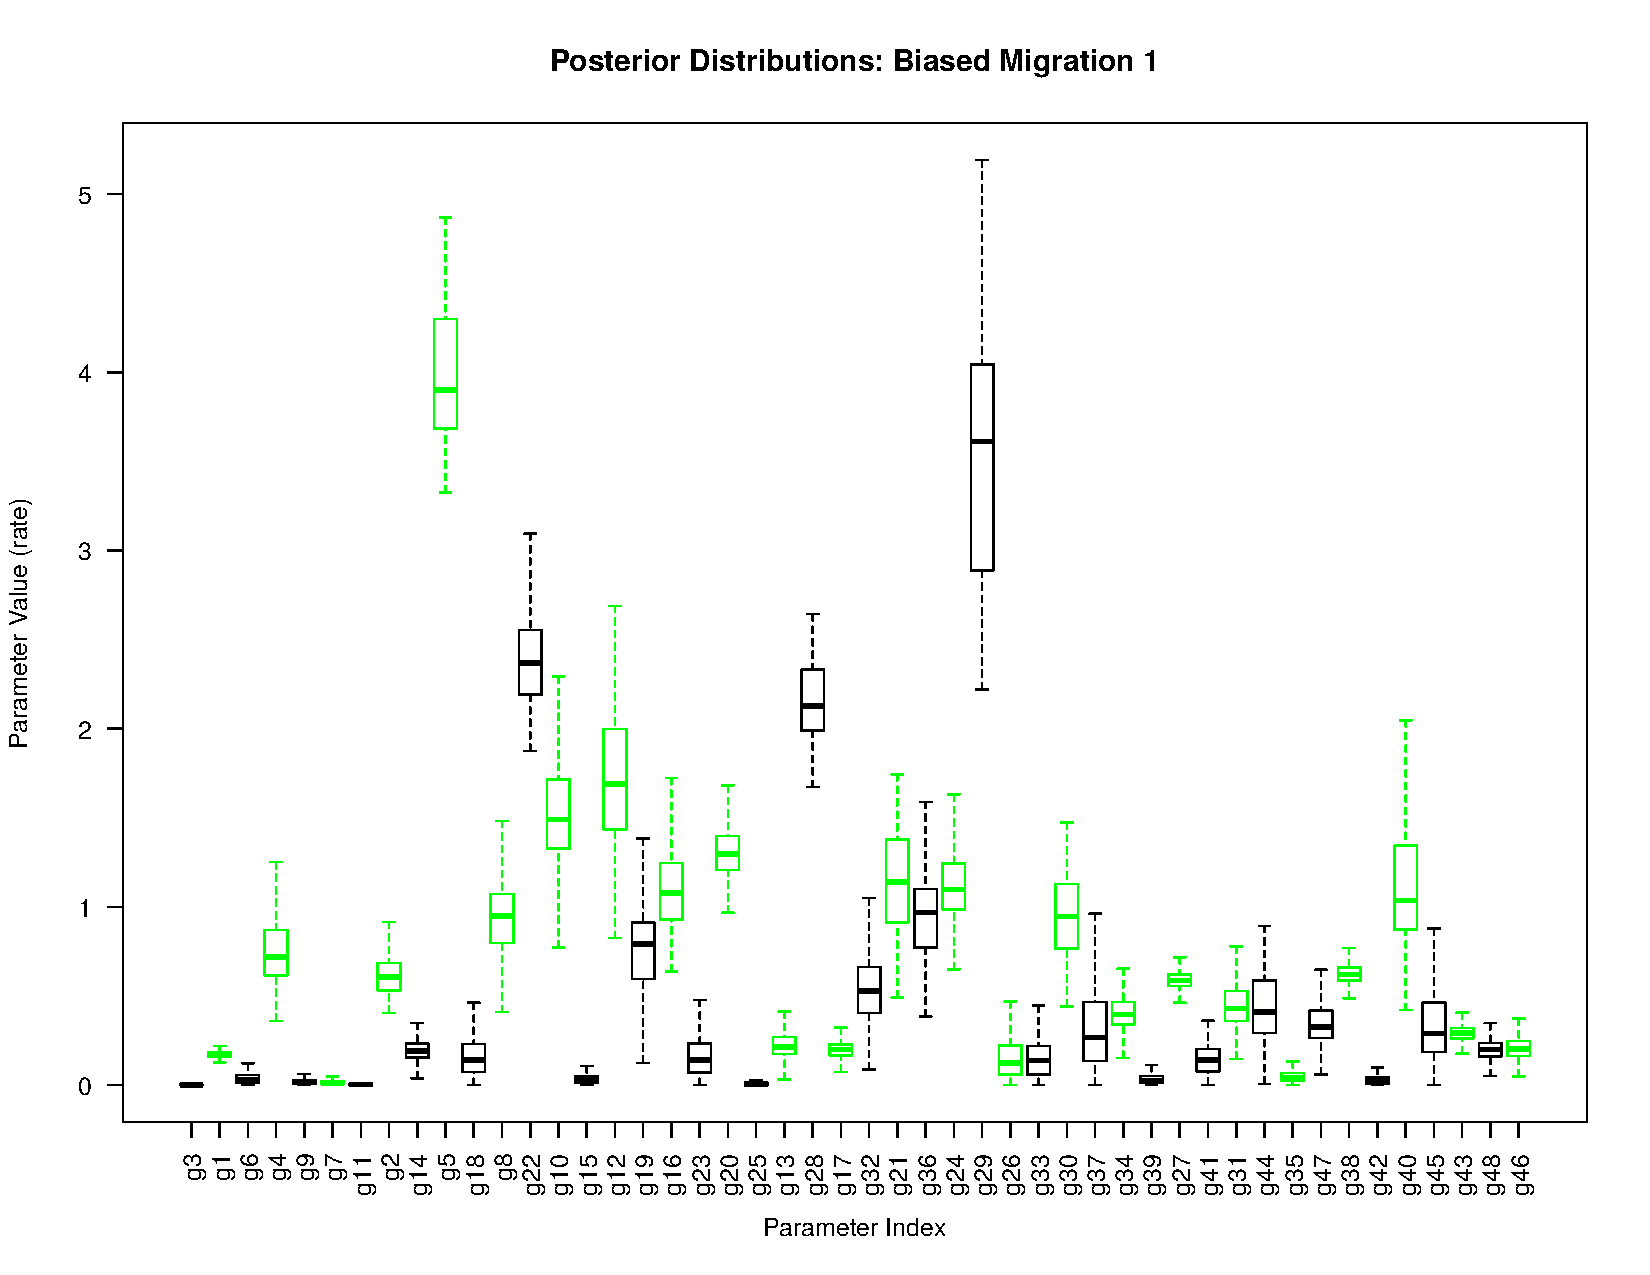
\includegraphics[scale=.6]{figs/post_dists_bias_4x4_1}
\caption{Boxplots of the posterior distributions for $g$ 
for the first replicate of the $4 \times 4$ discretization of the square landscape with biased migration.
Black boxes are gene flow rates down and to the left 
with each green box being the corresponding gene flow rate up and to the right.}
\label{fig:post_dists_bias_4x4_1}
\end{figure}

\section*{Application to the Mojave Desert Tortoise}

The Mojave desert tortoise (\textit{Gopherus agassizii})
lives across much of the Mojave desert of California and Nevada,
separated from its sister taxa, \textit{Gopherus morofkaii} by the Colorado river.
We applied our method to genomic distances calculated from
whole genome sequencing data of 271 individuals sampled from across much of the range,
reported in \citet{shaffer2017desert}.
We discretized the landscape into 13 regions based on watershed polygons
from the Watershed Boundary Dataset \citep{WBD}
(using WBD8 slightly modified by portions of WBD10 to improve contiguity of regions).
The resulting discretization,
overlaid on a map including tortoise sampling locations,
is shown in Figure \ref{fig:tort_land}.
Since the regions vary substantially in size, 
and may vary substantially in population density, 
we do not assume that coalescence rates are the same everywhere, 
which gives 13 coalescence rates;
combined with the 50 migration parameters between each pair of adjacent regions
we have a total of 63 unknown parameters
(and 91 equations).

Posterior distributions of the parameters are shown in Figure \ref{fig:tort_post}.
There is substantial variation in the gene flow rates 
but not the coalescence rates, 
with the exception of region 4, which seems to have a relatively slow coalescence rate.
This is not too surprising given its large area and central location.
Gene flow rates are low across mountainous boundaries:
for instance, regions 1 and 4 are separated by the Paiute and Castle mountains,
and regions 4 and 12 are separated by the Providence and Granite mountains.
% and regions 1 and 9 are separated by the New York and McCollough mountains.
On the other hand, there is a large, mostly open bajada connecting areas 9 and 13, 
and we infer high rates of migration between the two regions.
The coalescence time model provides a good fit to the data,
much better than was obtained by commute times, either \plr{in this paper??}
or using the resistance distance method of \citet{shaffer2017desert}
(Figure \ref{fig:tort_h_comp}).

The most biologically interesting aspects
are the strong asymmetries, for instance between region 9 and regions 11, 12, and 13.
These indicate that resistance-based methods may be strongly misled.
However, we cannot conclude from this analysis \emph{what} is leading to the observed asymmetries.
One explanation would be source-sink dynamics:
for instance, the observed bias in lineage movement could be observed 
if the tortoise fecundity in the Ivanpah valley in region 9
is higher than in the colder, higher-elevation regions to the north.
Or, it could be the result of a historical range expansion out of the area,
perhaps out of a more resticted range as climates changed after the last glacial maximum.
The presence of source-sink dynamics would be of great interest for tortoise conservation efforts,
but it is not clear from this analysis which explanation is more likely.
Some aspects of the results may even be the produced by sample configuration:
for instance, perhaps the inferred gene flow between regions 2 and 3 is low
simply because individuals sampled in region 3 are geographically far from region 2.

\begin{figure}
\centering
 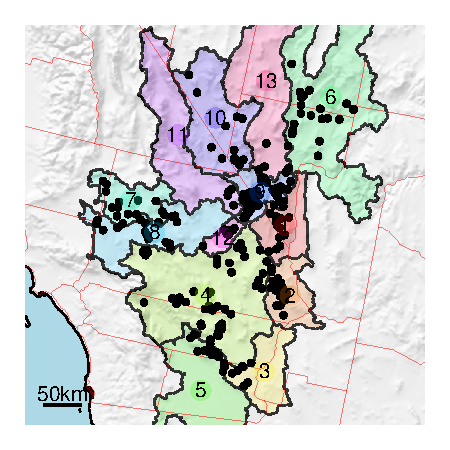
\includegraphics[width=0.45\textwidth]{figs/fancy_watershed_assignments}
 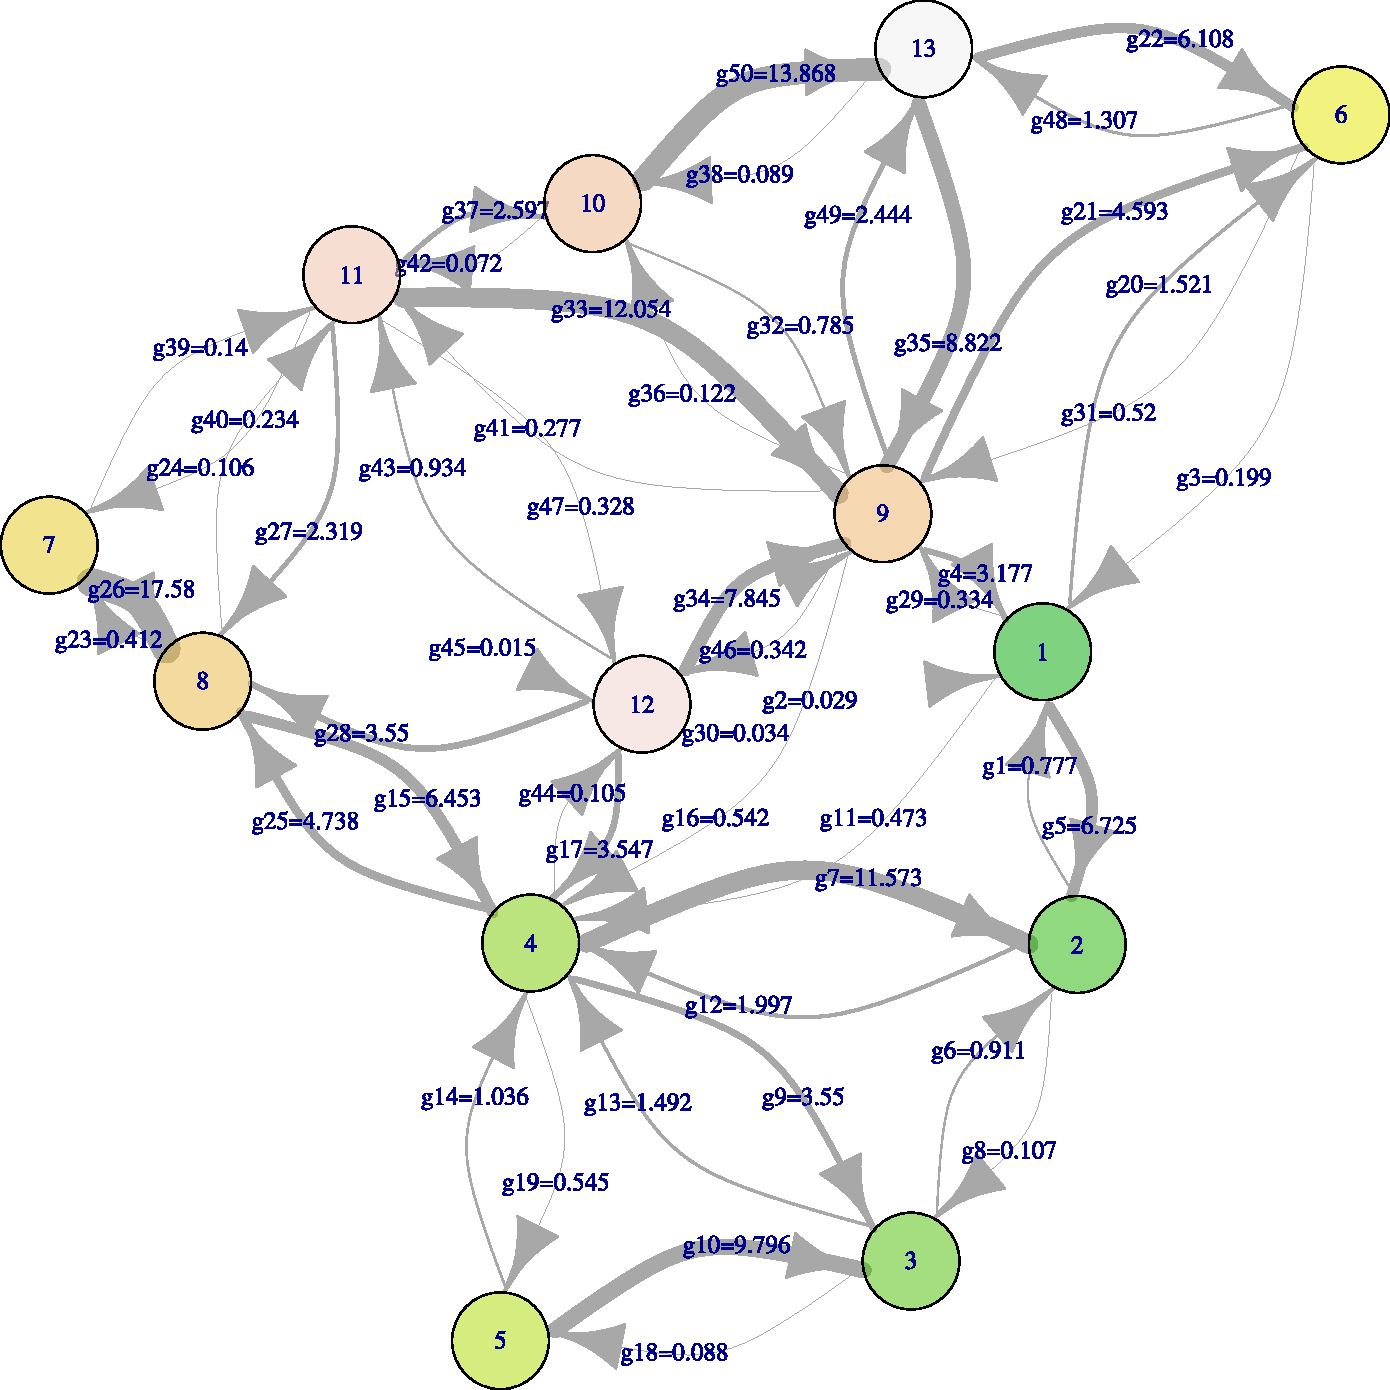
\includegraphics[width=0.45\textwidth]{figs/tort_graph_results}
\caption{Left: Locations of the sampled tortoises.
    \plr{add mountain shadings and ocean; remove bits on the other side of the Colorado}
    Right: Sample maximum posterior estimates 
    of movement rates.
    \plr{can these be maximum posterior estimates instead?}
    } \label{fig:tort_land}
\end{figure}

\begin{figure}
\centering
 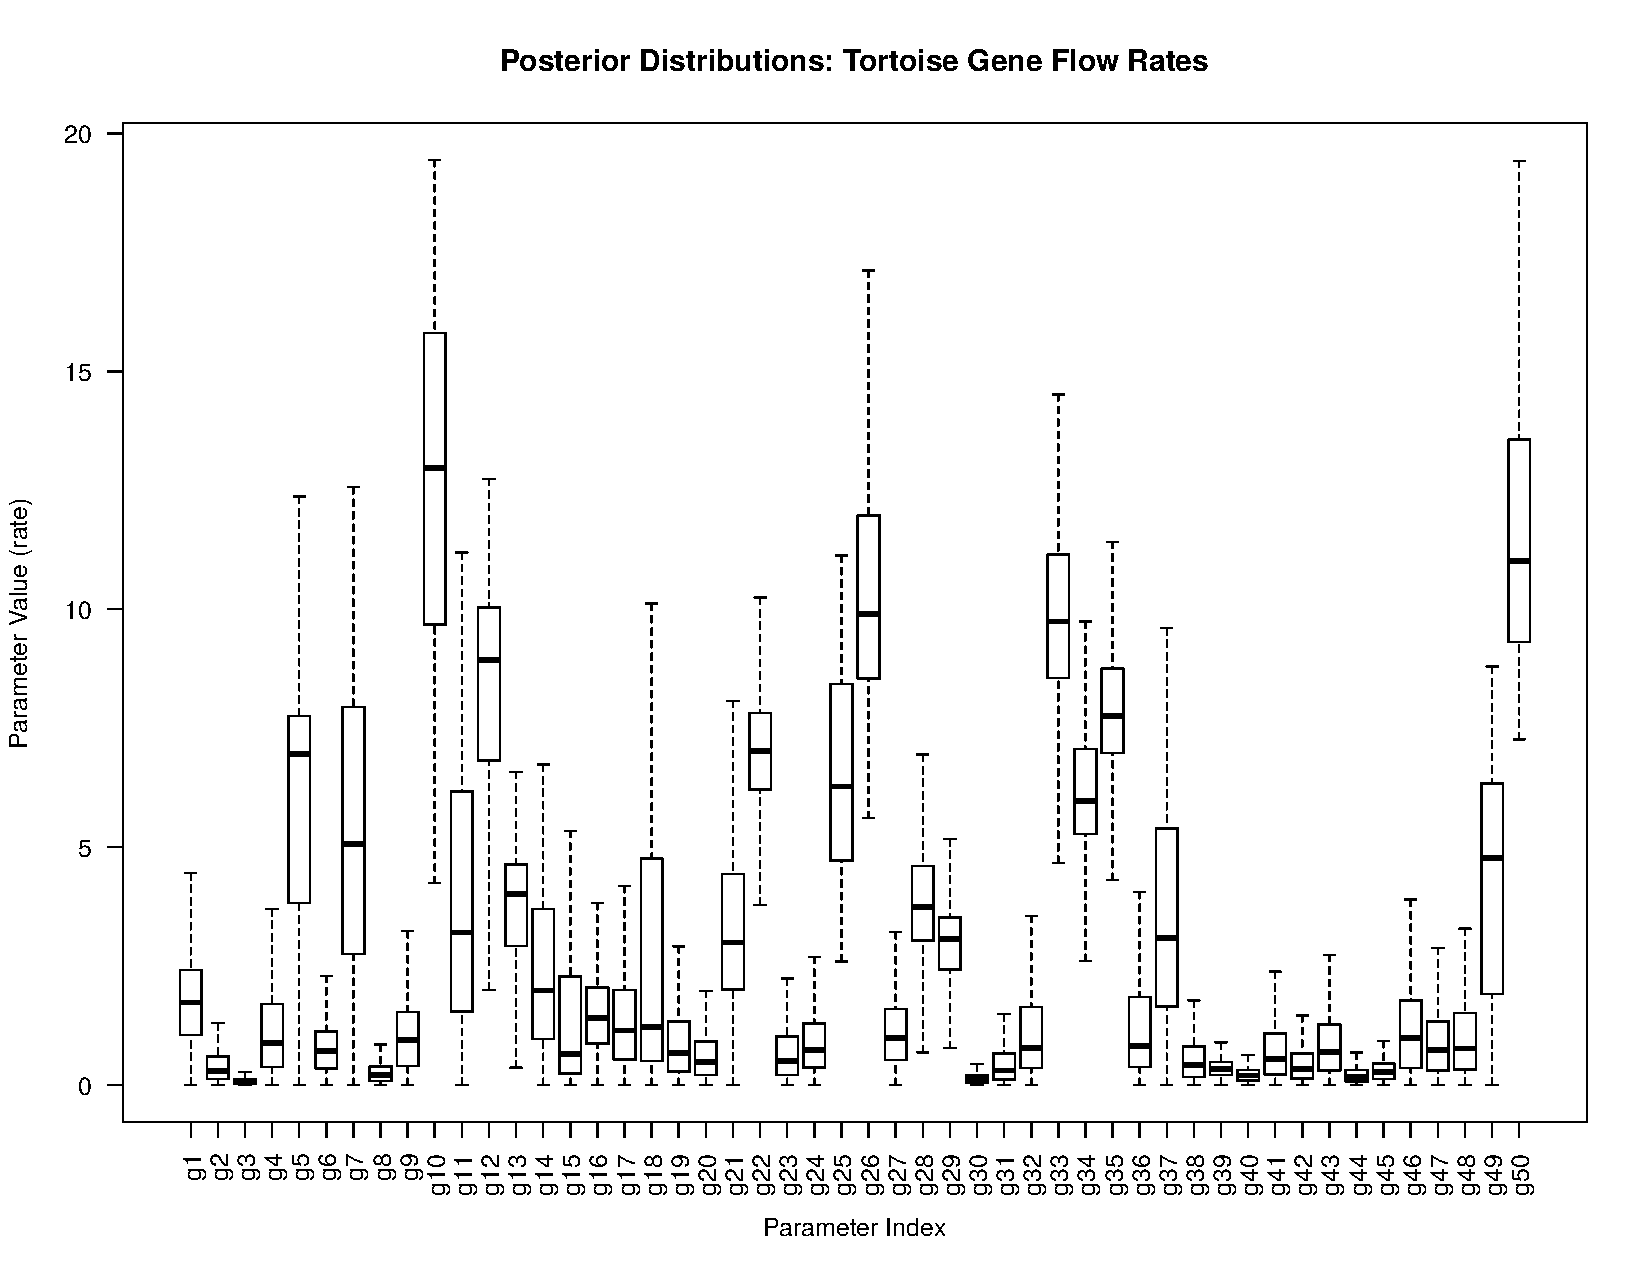
\includegraphics[width=0.8\textwidth]{figs/tort_post_g}
 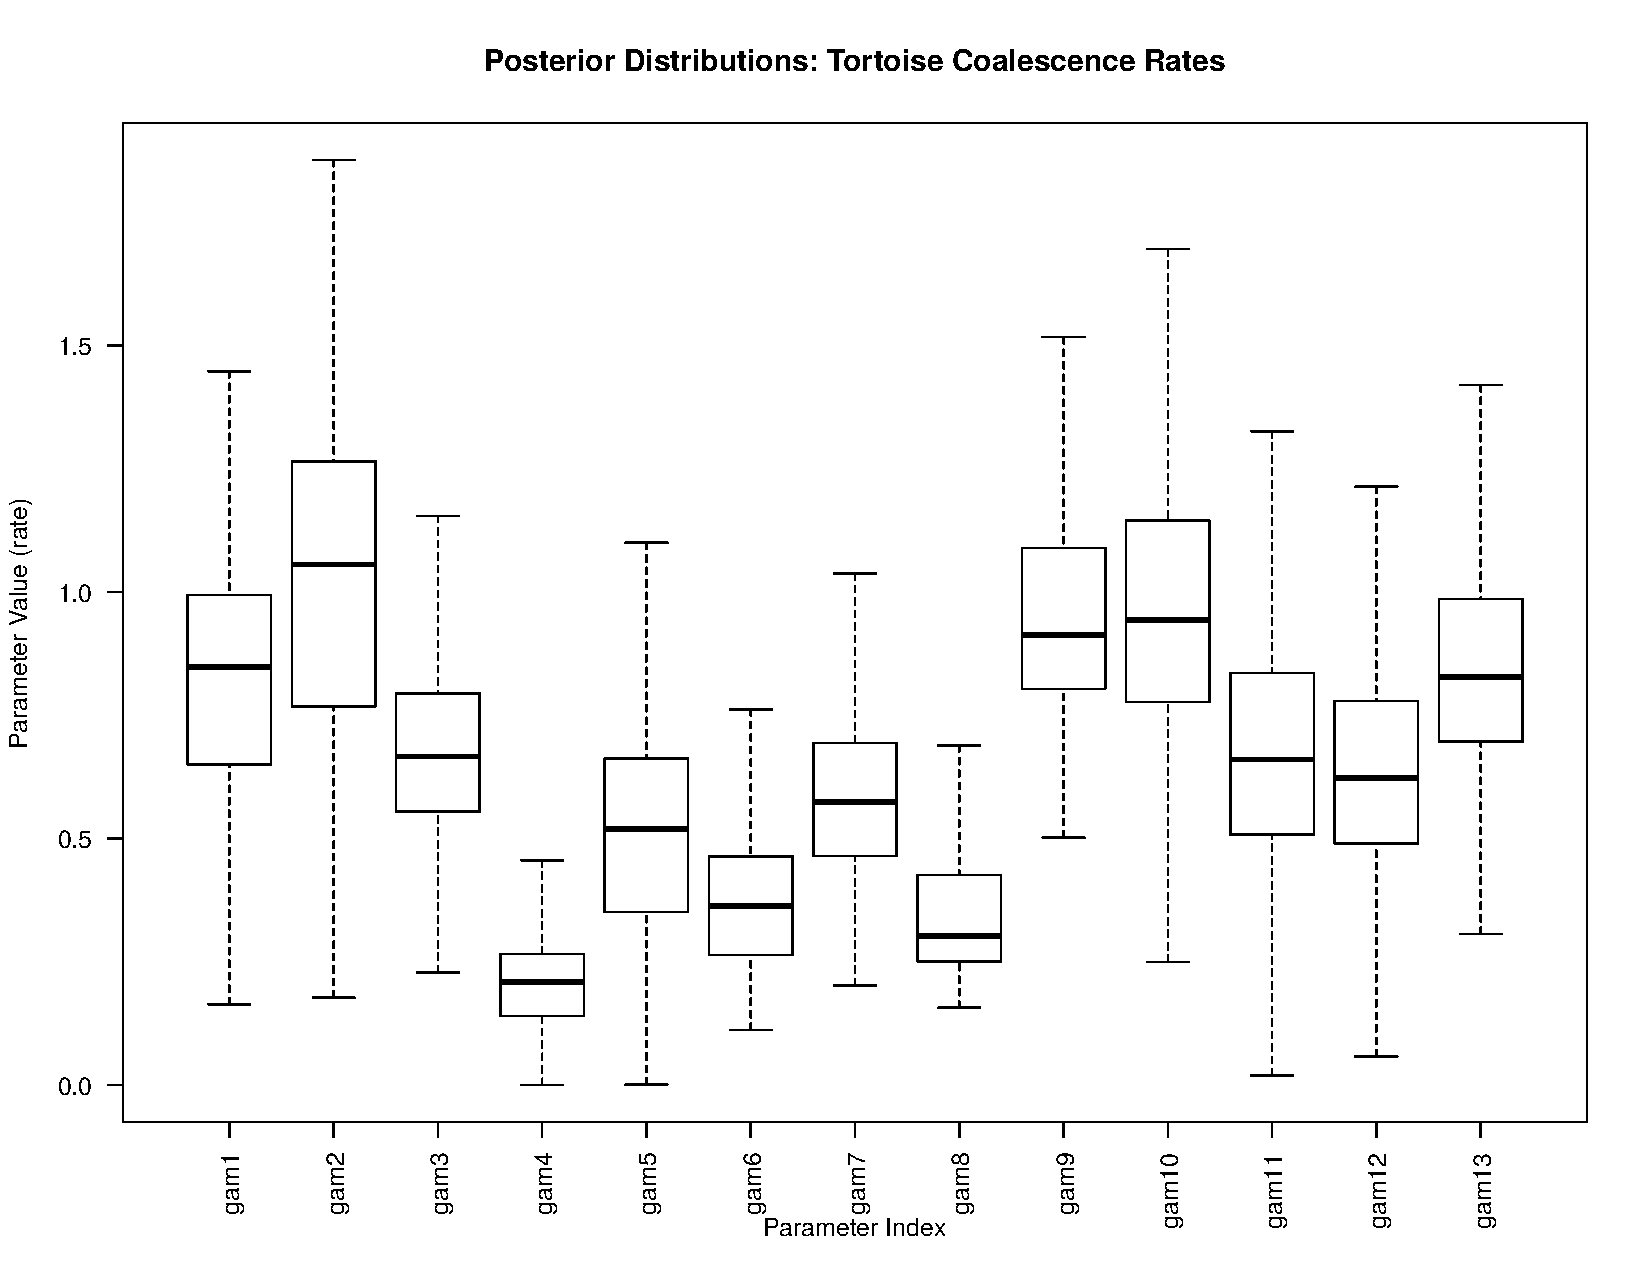
\includegraphics[width=0.8\textwidth]{figs/tort_post_gam}
\caption{
    Boxplots of the posterior distributions for 
    \textbf{(top)} movement rates, and
    \textbf{(bottom)} coalescence rates,
    for the Mojave desert tortoise data set.
    Parameters are labeled as in Figure \ref{fig:tort_land}.
    } \label{fig:tort_post}
\end{figure}

\begin{figure}
\centering
 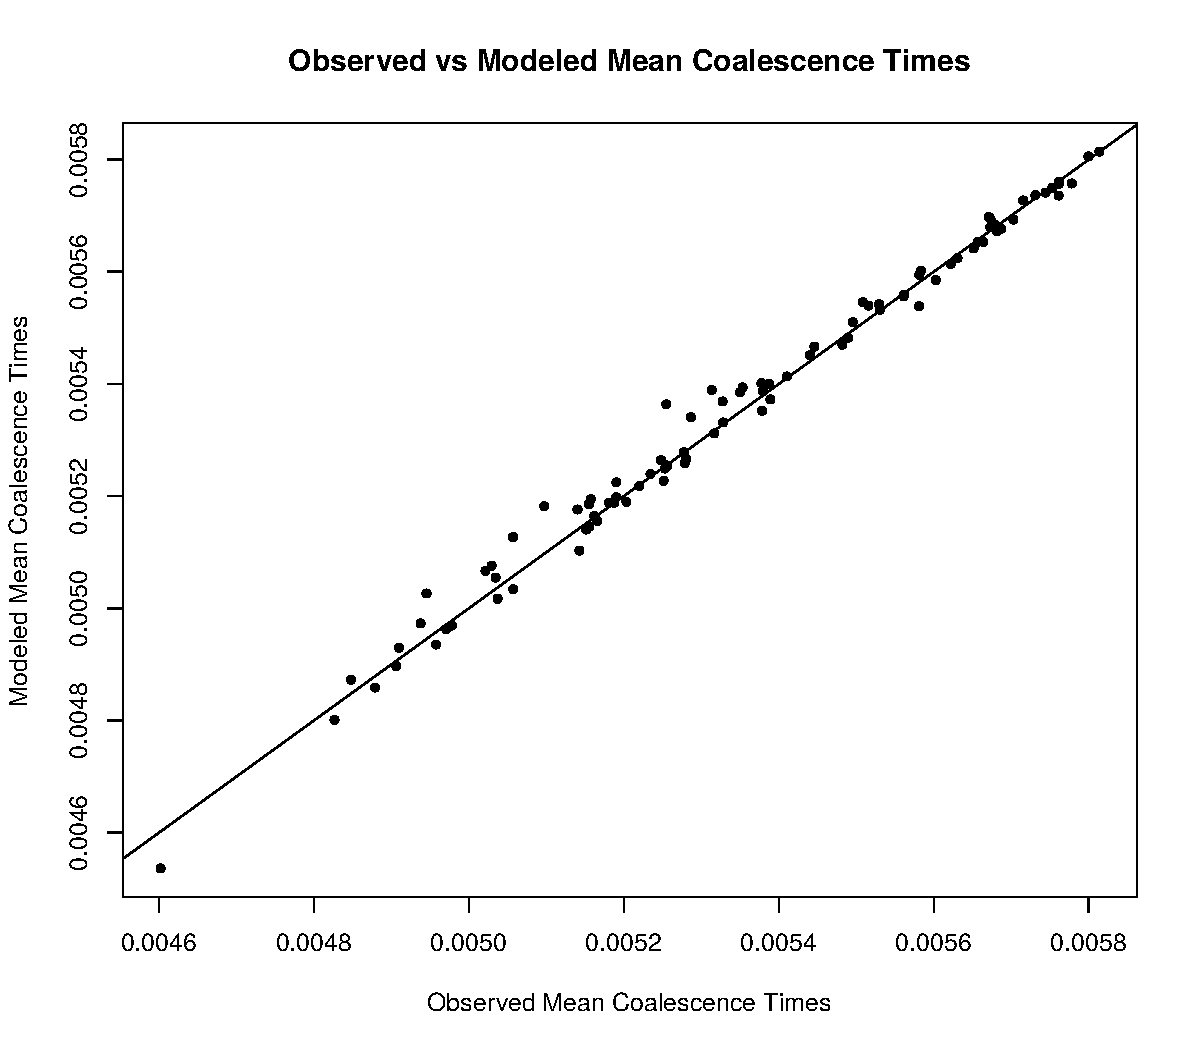
\includegraphics[scale=.8]{figs/tort_h_comp}
\caption{
    Mean coalescence times calculated from the sample maximum likelihood model parameters 
    plotted against the observed mean coalescence times calculated from the tortoise data, 
    measured in the mean of pairwise $\pi$.
    The mean absolute value relative differences between the two is 0.4\%.
    } \label{fig:tort_h_comp}
\end{figure}


%%%%%%%%%%%%%%%%%%%%
\section*{Discussion}

With these methods, we provide a framework for
inferring demographic parameters of 
populations living on a habitat spread over a two dimensional landscape 
by using present day location and genetic sequencing information.
We are able to do inference of reverse time gene flow and coalescence rates 
with the matrix of mean coalescence times
in cases where the matrix is noise-free, noisy, or incomplete, 
or when it made after discretization of a simulated or real landscape.
To do this, we assume that the reverse time movements of lineages are Markov
and the population is near stationarity.
Typically, there is more error and uncertainty in the posterior distributions of the parameters
when there is more noise, slower coalescence rate, more missing values,
and multiple parameters for coalescence rate.

In addition to developing a method for inferring migration rates using pairwise coalescence times,
we compare the results with that of resistance distance (i.e., commute time) based inference.
Coalescence based inference typically has lower error than commute time based inference,
along with the benefit that you can also infer coalescence rates. 
The commute time plus diversity estimate, $\comdist$, 
provides a good estimate of the coalescence times, $C$,
when gene flow rates are symmetric ($G_{ij} = G_{ji}$), 
but can be very wrong when they are asymmetric, 
including extreme discrepencies 
when there is an overall bias in the direction of the asymmetry across the landscape 
(Figure \ref{fig:RvsC}).
When inference is performed on discrete landscapes 
with varying degrees of migrational asymmetry, 
coalescence time based inference is more accurate than commute time inference in all tested cases
(Figure \ref{fig:4x4box}).
Although performance of the commute time based method is reasonable 
when gene flow rates in the underlying model are symmetric, 
it becomes worse as the gene flow rates become more asymmetric 
to the point where there is little correlation at all with the true values 
when there is biased asymmetric migration.
On the other hand, commute time inference is much less computationally intensive, 
so much larger spatial systems can be used.
If the gene flow rates are symmetric, the higher resolution allowed by commute time inference
may outweigh the loss in accuracy.
The implication of these results for the body of literature using resistance distance methods
is that one may need to use caution when interpreting results.
For example, inferring high gene flow rates between two areas by using resistance distance
could potentially mean that those were areas were actually being fed by a common source.
Therefore, it may be worthwhile to apply a coarse resolution coalescence time based method 
alongside a finer resolution resistance distance method 
in order to check for evidence of asymmetric gene flow patterns.

Although commute and coalescence times can be quite different,
we show that they are equal (with a particular choice of local diversity)
if populations are arranged on a ring or torus
with symmetric migration.
The similarity of these models to rectangular grids
may explain why in other work, commute time methods have shown relatively good fit to data
simulated with symmetric migration rates.

We also apply the method to data from continuous space simulations. 
While there is substantial variation between the inferred values 
for different simulations with the same underlying demographic parameters, 
we are able to reliably find evidence of biased asymmetric migration (if it is present)
and verify the exitence of a barrier to migration, 
even when the landscape is otherwise relatively well connected.
Further work could involve more precise study of the relationship
between reverse time gene flow rates and forwards time migration rates.

\paragraph{Asymmetric dispersal}
(Review of asymmetric situations.)

\citet{hanks2017modeling} developed a method that allows asymmetry
by modeling genetic similarity as deriving from an underlying random field
whose space-time covariance is given by the covariance of the (forwards-time) population fluctuations.


\paragraph{Consequences for resistance methods}
We have shown that commute time can show dramatically different patterns
than coalescence time, especially if there is systematic bias in dispersal.
How should this affect the results of resistance-based methods to genomic data,
besides general inaccuracy?
Suppose, for instance, that seed dispersal for a species of tree
is biased downhill,
and the landscape is dominated by a large valley.
Since lineages tend to move uphill,
genetic distance between locations on opposite slopes of the valley will be relatively large,
so resistance methods will infer a barrier along the bottom of the valley
when no barrier to dispersal exists.
On the other hand, if there is a ridge instead of a valley,
resistance methods will show no barrier (and relatively high movement rates),
even if there is very little uphill dispersal.
This could lead to a falsely high assessment of gene flow across the top of the ridge.
\plr{Also applies to least-cost path analysis.}

\paragraph{Circuitscape}
Could we use coalescence time in place of commute time
for workflows that compute values on a given map of movement rates
that are then compared to genetic distance?
In principle this could be done,
but not at the same (impressively fine) geographic resolution that is currently possible,
e.g., using Circuitscape \citep{circuitscape}.
This is because if we have $n$ sampled locations
on a landscape discretized into $N$ regions,
the computational complexity of finding commute times is $nN$,
but coalescence time scales as $N^2$.
This is because each $N$-vector of hitting times to a particular location can be found independently,
but the entire $N \times N$ matrix of coalescence times must be found together.
However, as we discuss above, this fine geographic resolution is in some sense illusory --
for each fine-resolution map there should be coarser maps that give almost identical coalescence times.
However, we are not aware of existing theory providing guidance on how to find these.

\paragraph{Difficulty of inference}
What determines the feasability of inferring movement rates from genetic distances?
Using coalescence times instead of commute times greatly improves accuracy in many situations,
but there are still a number of factors that determine the tractability of the problem.
Observation noise is clearly an issue;
we found that estimation errors of a few percent was enough to seriously degrade accuracy.
However, genetic distances can be estimated to much higher accuracy using modern genomic data.
Perhaps more seriously,
a rate of coalescence relative to movement can also make the problem essentially nonidentifiable.
This is clear at least in the limit: with very low coalescence, 
the population loses any isolation by distance and looks panmictic.
In continuous landscapes, this balance is measured by Wright's local effective population size,
which is proportional to the number of other individuals 
within a circle of radius equal to the mean dispersal distance.
\plr{more about continuous landscapes and discretization}

\paragraph{The effect of history}
The models we discuss here assume that population sizes and migration rates
have been constant on the time scale given by the within-species coalescent time.
This is rarely true in practice \citep{avise,barton}.
However, geographic differences in mean relatedness
are established on a shorter time scale --
the time scale over which a lineage, moving randomly across the landscape,
``forgets'' where it started
(i.e., the mixing time of the Markov chain).
This is the time it takes for the uncertainty in lineage movement
to reach the scale of the species range.
For instance,
the width of the tortoise range is roughly 500km,
and if mean dispersal distance is 10km (a high estimate),
the standard deviation of ancestor location $t$ generations ago is $10\sqrt{t}$,
so the mixing time of tortoise lineages across the modern landscape,
not accounting for barriers, is of order 2500 generations,
or about 50,000 years.
The landscape of the Mojave has changed substantially over tihs time \citep{pleistocene_mojave},
which suggests that models incorporating change over time 
may be required to model modern tortoise diversity.
However, the effects of recent history are strongest,
so landscapes estimated assuming constant populations
may give a reasonable picture of the landscape averged over recent times.

\paragraph{Limitations of data}
Something about microsats versus RADseq versus whole-genome.
\plr{XXX}

\paragraph{Landscapes or discrete demes?}
Other inference methods \citep{wilson2003bayesian,beerli1999maximum,beerli2010unified,hey2007integration}
work with coalescence inference, but only with a small number of loci and populations,
because of computational efficiency.
We're somewhere in between.
\plr{XXX}


\paragraph{Assumptions}
Modeling lineages as a Markov chain is nearly ubiquitous in population genetics today,
but may not be appropriate.
Even though the population dynamics in forwards time are Markov, the dynamics of lineages traced back
in time (the coalescent process) may not be. For example, if fecundity is variable and population density
is low, two lineages near each other are more likely to share a recent common origin, so knowing how one
lineage moves gives you information about how the other lineage is likely to move. This effect becomes
negligible as population density increases [Barton et al., 2002]), so it should not be an issue if the offspring
of any one parent are typically interspersed with the offspring of many others. The methods I develop here
model the coalescent process as Markov, which should be a good approximation for many systems.

\paragraph{other points:}
Practical example (tortoises) shows strong asymmetry.
Methods dealing with ill-posedness are necessary.
Other measures of genetic distance: what do people use in practice?


%%%%%%%%%%%%%%%%%%%%%%%%%%%
\section*{Acknowledgements}

Thanks to David Levin for useful suggestions regarding hitting time calculations,
to Paul Marjoram for useful comments,
and to Brad Shaffer and Evan McCartney-Melstad for useful discussions
and providing the genetic distance data for desert tortoises.
We are also indebted to Chava Weissman, Bridgette Hagerty, Fran Sandmeier, Dick Tracy,
and a large number of field workers for collecting the original tortoise tissue samples.
\plr{also John, Hossein, Desi, ??}


\bibliography{references}

\appendix
\renewcommand{\thefigure}{S\arabic{figure}}
\setcounter{figure}{0}


%%%%%%%%%%%%%%%%%%%%%%%%%%%%%%
\section{Finding $G$ from $H$}
\label{apx::hitting_calcs}

\plr{edit}

Suppose that $G$ is the generator matrix of an irreducible continuous-time Markov chain $X$,
so that $G_{ij} \ge 0$ for $i \neq j$ and
$$ G 1 = 0 $$.

Let $\tau_{j} = \inf\{t \ge 0 : X_t = j\}$ and $H_{ij} = \E[\tau_j \,|\, X_0 = i]$.
Then we know that
$$
    (G H)_{ij} = -1 \qquad \text{for} \; i \neq j ,
$$
i.e.,
\begin{align} \label{eqn:GH}
    GH = - 1 1^T + \diag(x).
\end{align}

What is $x$?  Well, note that
$$
    G = (\diag(x) - 1 1^T) H^{-1}
$$
and so
$$ \begin{aligned}
    0 &= G1 \\
    &= (\diag(x) - 1 1^T) H^{-1} x 
\end{aligned} $$
and so
$$
    x_i = \frac{ 1^T H^{-1} 1 }{ (H^{-1} 1)_i } .
$$
Furthermore,
the Random Target Lemma \citep{aldous} % https://www.stat.berkeley.edu/users/aldous/RWG/Book_Ralph/Ch2.S2.html
tells us that if $\pi$ is the stationary distribution of the chain, then 
$(H \pi)_i$ does not depend on $i$,
i.e., that $H \pi \propto 1$,
and thus if $H^{-1} 1 = \nu$, 
then $\pi = \nu / \sum_i \nu_i$.
This says exactly that $x_i = 1/\pi_i$.

In summary, $\pi = H^{-1} 1 / 1^T H^{-1} 1$, and 
\begin{align}
    G 
    &= (\diag(1/\pi) - 1 1^T) H^{-1} .
\end{align}
Note that this equation only specifies $H$ up to a constant added to each column:
i.e., if given $G$ one obtains a matrix $Y$ solving $GY = \diag(1/\pi) - 1 1^T$,
then $H_{ij} = Y_{ij} - Y_{jj}$.


%%%%%%%%%%%%%%%%%%%%%%%%%%%%%%
\section{Equality of commute and coalescence times}
\label{sec:com_eq_coal}

Under what conditions are coalescence times and commute times (with some local diversity values) equal?
In other words, for what choices of $G$, $\gamma$, and $q$ does
\begin{align}
    \comdist = (H + H^T)/4 + (q 1^T + 1 q^T)/2
\end{align}
solve equation \eqref{eqn:C_matrix}?
Writing this out, this says that
\begin{align} \label{eqn:R_coal}
    ( GH + (GH)^T + GH^T + (GH^T)^T )/4 + (Gq 1^T + 1 (Gq)^T)/2
    &=
    \diag(q) \diag(\gamma) - 1 1^T .
\end{align}
(To simplify this we used the fact that $\diag(H) = 0$ and $G1 = 0$.)

It is not clear what can be said about the general case because of the presence of $HG^T$,
but if we assume that $H$ is symmetric, we can make progress,
because then we have that $GH = GH^T$, 
and so equation \eqref{eqn:GH} says that all four terms in the first group are equal,
and equation \eqref{eqn:R_coal} simplifies to
\begin{align} \label{eqn:R_eq_C}
    \diag(1/\pi) + (Gq 1^T + 1 (Gq)^T)/2
    &=
    \diag(q) \diag(\gamma) ,
\end{align}
where the $-1 1^T$ terms on each side canceled.
Because $G1=0$,
the most obvious solution to this is if $q = c 1$ and $c \gamma = 1/\pi$, for some constant $c$
(although there is a broader family of solutions).

In summary, if hitting times are symmetric
and coalescence rates are equal to the inverse of the stationary distribution,
then coalescence times are equal to commute times plus one.
This is fairly restrictive, 
but does occur if the population configuration is isotropic
(as for instance in an all-connected-to-all island model with equal migration rates)
or in populations arranged around a ring
with migration rates depending only on the distance between them.

Can we solve equation \eqref{eqn:R_eq_C} more generally?
For that equation to hold, we need $Gq 1^T +  (Gq)^T$ to be diagonal,
i.e., that $(Gq)_i + (Gq)_j = 0$ for all $i \neq j$.
For any $k \neq \ell$, there exists a vector $u^{(k\ell)}$ such that $(Gu^{(k\ell)})_i = \delta_{ik} - \delta_{i\ell}$;
the only possible $q$ for which $Gq 1^T +  (Gq)^T$ is diagonal
are of the form $q = \alpha 1 + \beta u^{(k,\ell)}$ for some $k \neq \ell$ and some constants $\alpha$ and $\beta$.
We would then need
\begin{align}
    1/\pi_i + \delta_{ik} - \delta_{i\ell} = q_i \gamma_i \qquad \text{for all} i.
\end{align}
This implies that for any Markov chain with symmetric hitting times,
we can find diversity values ($q$) and coalescence rates ($\gamma$) that make $\comdist = C$
(and in fact there are many ways to do this).
However, there is not a general solution for $q$ if coalescence rates are also given (as is the case in practice).

%%%%%%%%%%%%%%%%%%%%%%%%%%%%%
\subsection*{Something else?}

\citet{strobeck1987average} showed that $\diag(C)$ was constant and does not depend on movement rates
for any isotropic conservative migration model.
Can we explain this?
(Also cite earlier.)


%%%%%%%%%%%%%%%%%%%%%%%%%%%%%%
\section{Further inference results}

Here we put some more plots describing inference method accuracy.


\begin{figure}
\centering
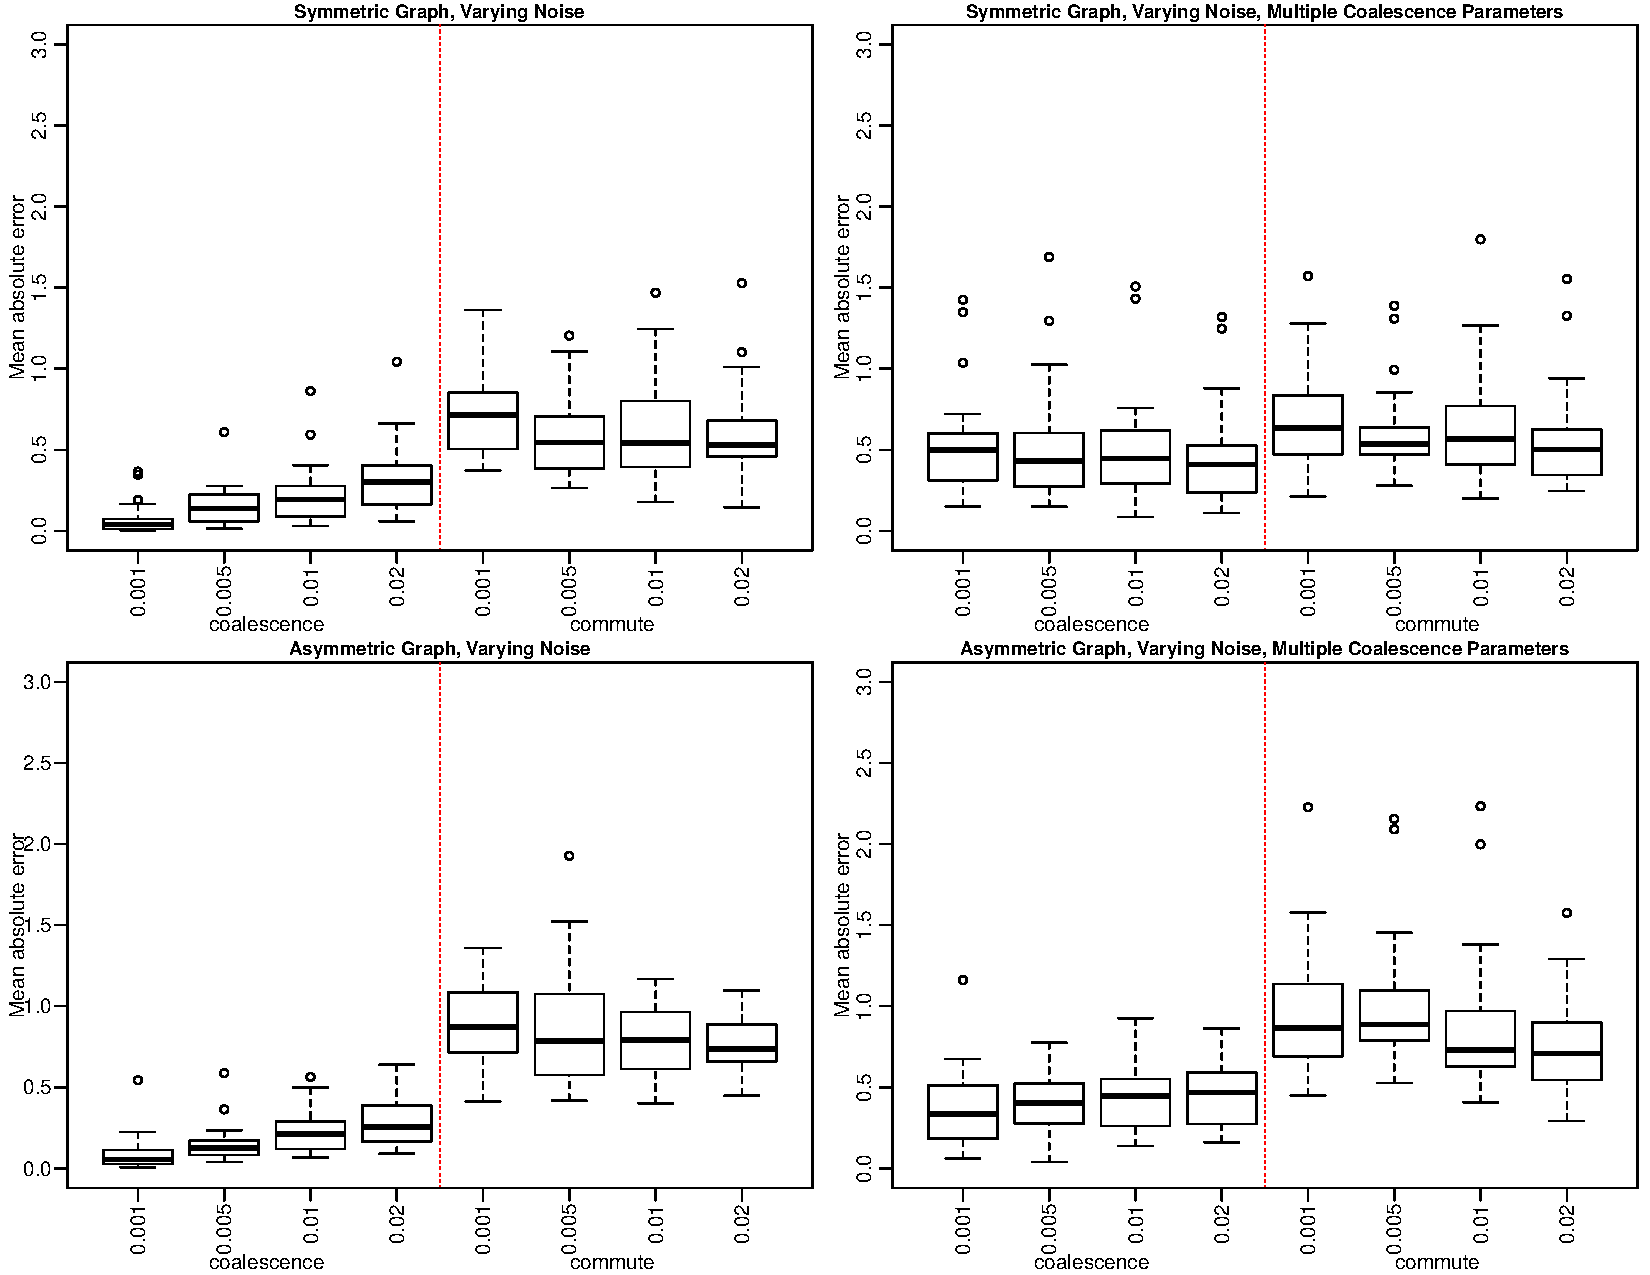
\includegraphics[scale=.6]{figs/mult_noise}
\caption{Boxplots of the mean absolute error, %in $\hat{g}$.
defined to be the absolute value difference between the true value and posterior median,
averaged across movement parameters $g$ for each of the 25 graphs in each situation.
Each box is labeled with the relative amount of noise added to $H$ to make $\hat{H}$.
The top left shows the results for symmetric graphs 
when there is a single coalescence parameter for all locations,
the top right for symmetric graphs 
when there is a separate coalescence parameter for each location,
the bottom left for asymmetric graphs 
when there is a single coalescence parameter for all locations,
and the bottom right for asymmetric graphs 
when there is a separate coalescence parameter for each location.}
\label{fig:mult_noise}
\end{figure}

\begin{figure}
\centering
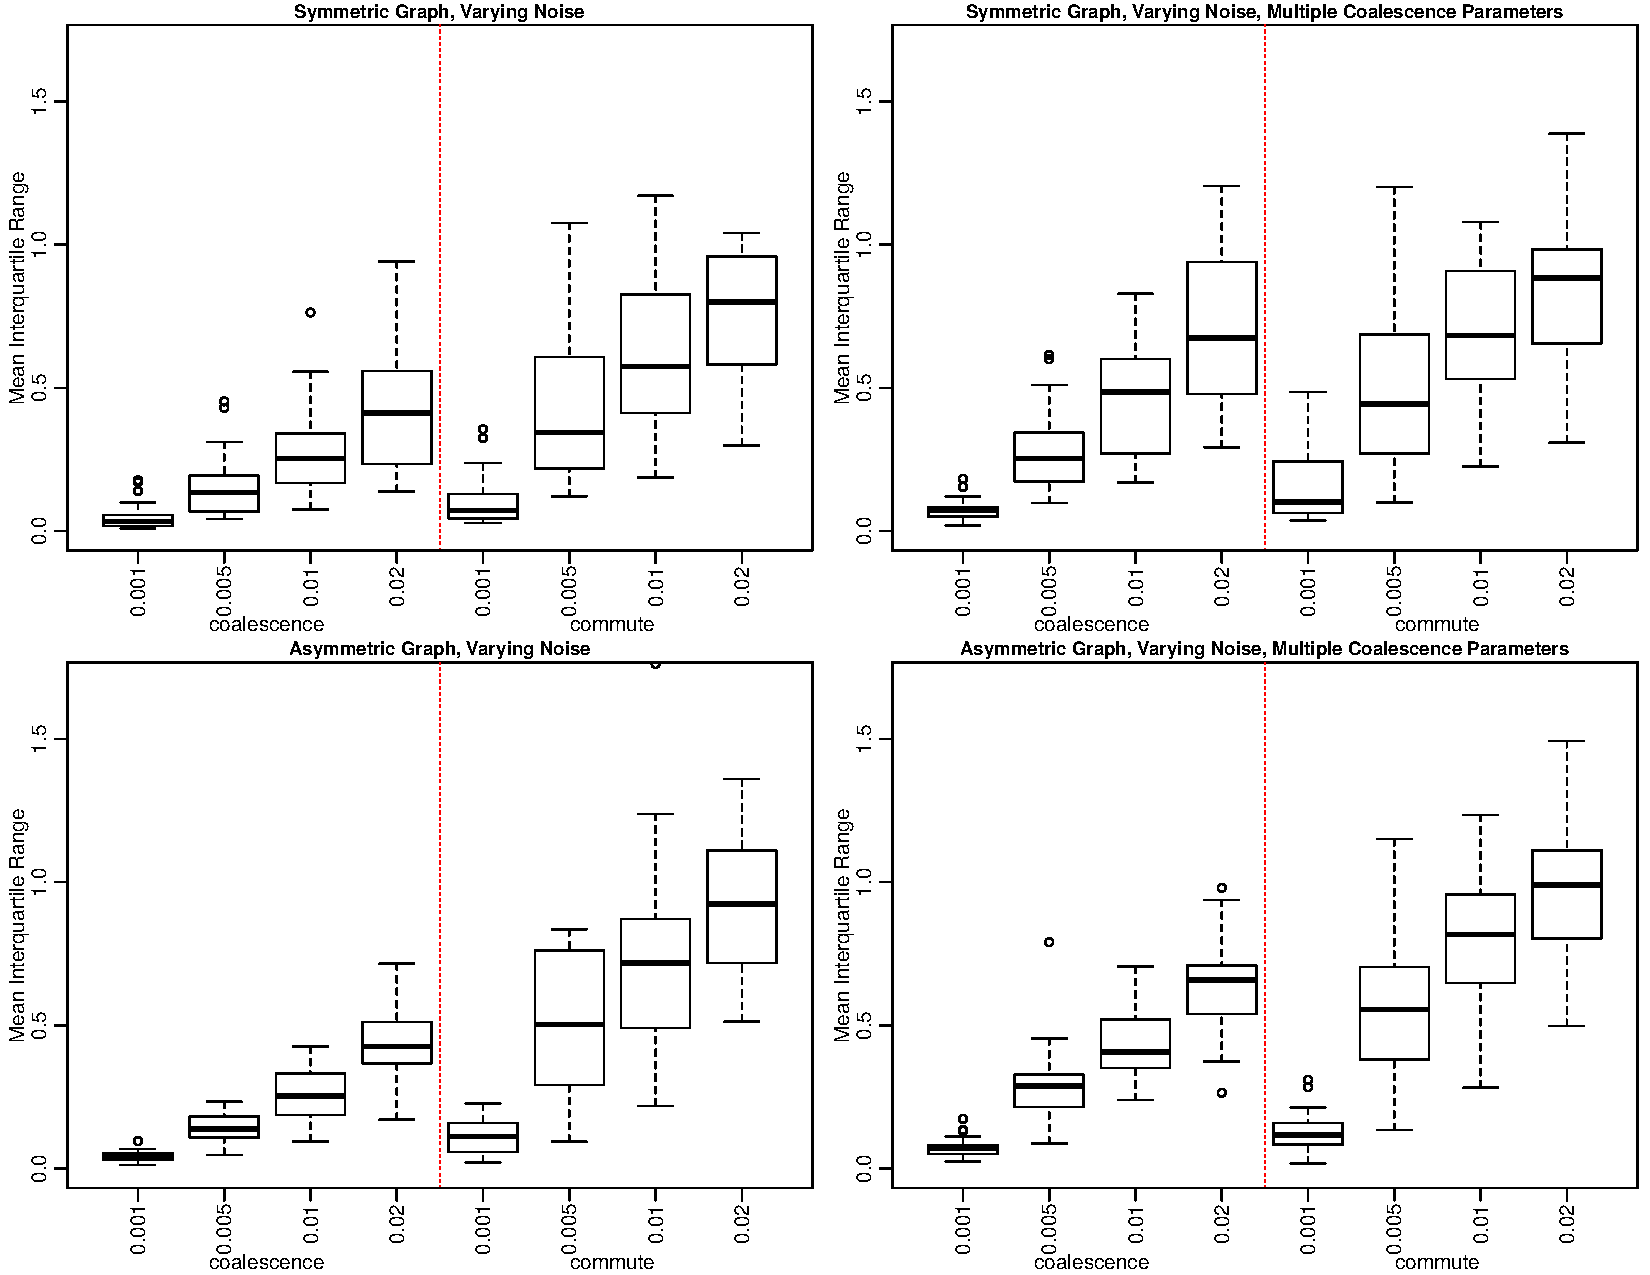
\includegraphics[scale=.6]{figs/mult_noise_iqr}
\caption{Boxplots of the mean interquartile ranges of the posterior distributions of $g$
for each of the 25 graphs in each situation.
Each box is labeled with the relative amount of noise added to $H$ to make $\hat{H}$.
Subplot locations for each situation are the same as in Figure \ref{fig:mult_noise}.
%The top left shows the results for symmetric graphs 
%when there is a single coalescence parameter for all locations,
%the top right for symmetric graphs 
%when there is a separate coalescence parameter for each location,
%the bottom left for asymmetric graphs 
%when there is a single coalescence parameter for all locations,
%and the bottom right for asymmetric graphs 
%when there is a separate coalescence parameter for each location.
}
\label{fig:mult_noise_iqr}
\end{figure}


\begin{figure}
\centering
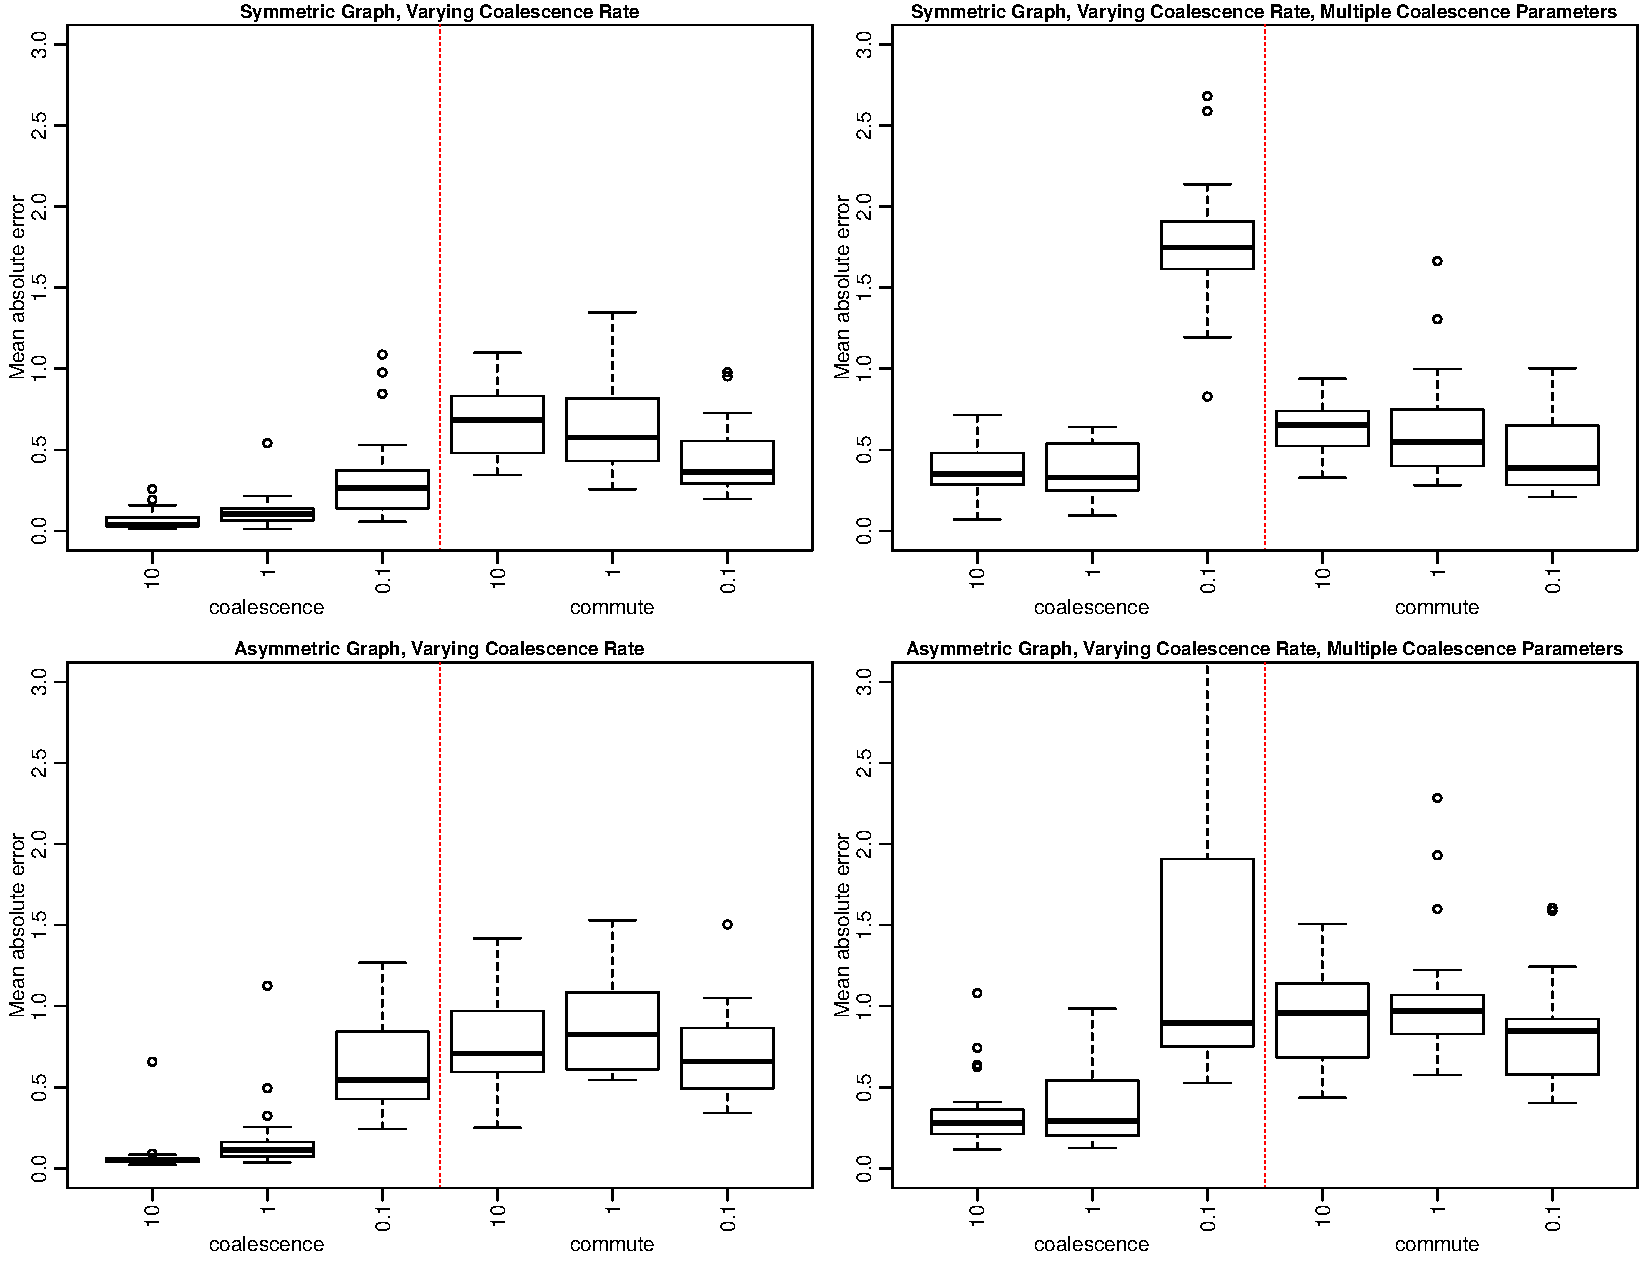
\includegraphics[scale=.6]{figs/mult_gam}
\caption{
Boxplots of the mean absolute error, %in $\hat{g}$.
defined to be the absolute value difference between the true value and posterior median,
averaged across movement parameters $g$ for each of the 25 graphs in each situation.
Each box is labeled with the coalescence rate in the underlying model for each situation.
Subplot locations for each situation are the same as in Figure \ref{fig:mult_noise}.
%The top left shows the results for symmetric graphs 
%when there is a single coalescence parameter for all locations,
%the top right for symmetric graphs 
%when there is a separate coalescence parameter for each location,
%the bottom left for asymmetric graphs 
%when there is a single coalescence parameter for all locations,
%and the bottom right for asymmetric graphs 
%when there is a separate coalescence parameter for each location.
}
\label{fig:mult_gam}
\end{figure}

\begin{figure}
\centering
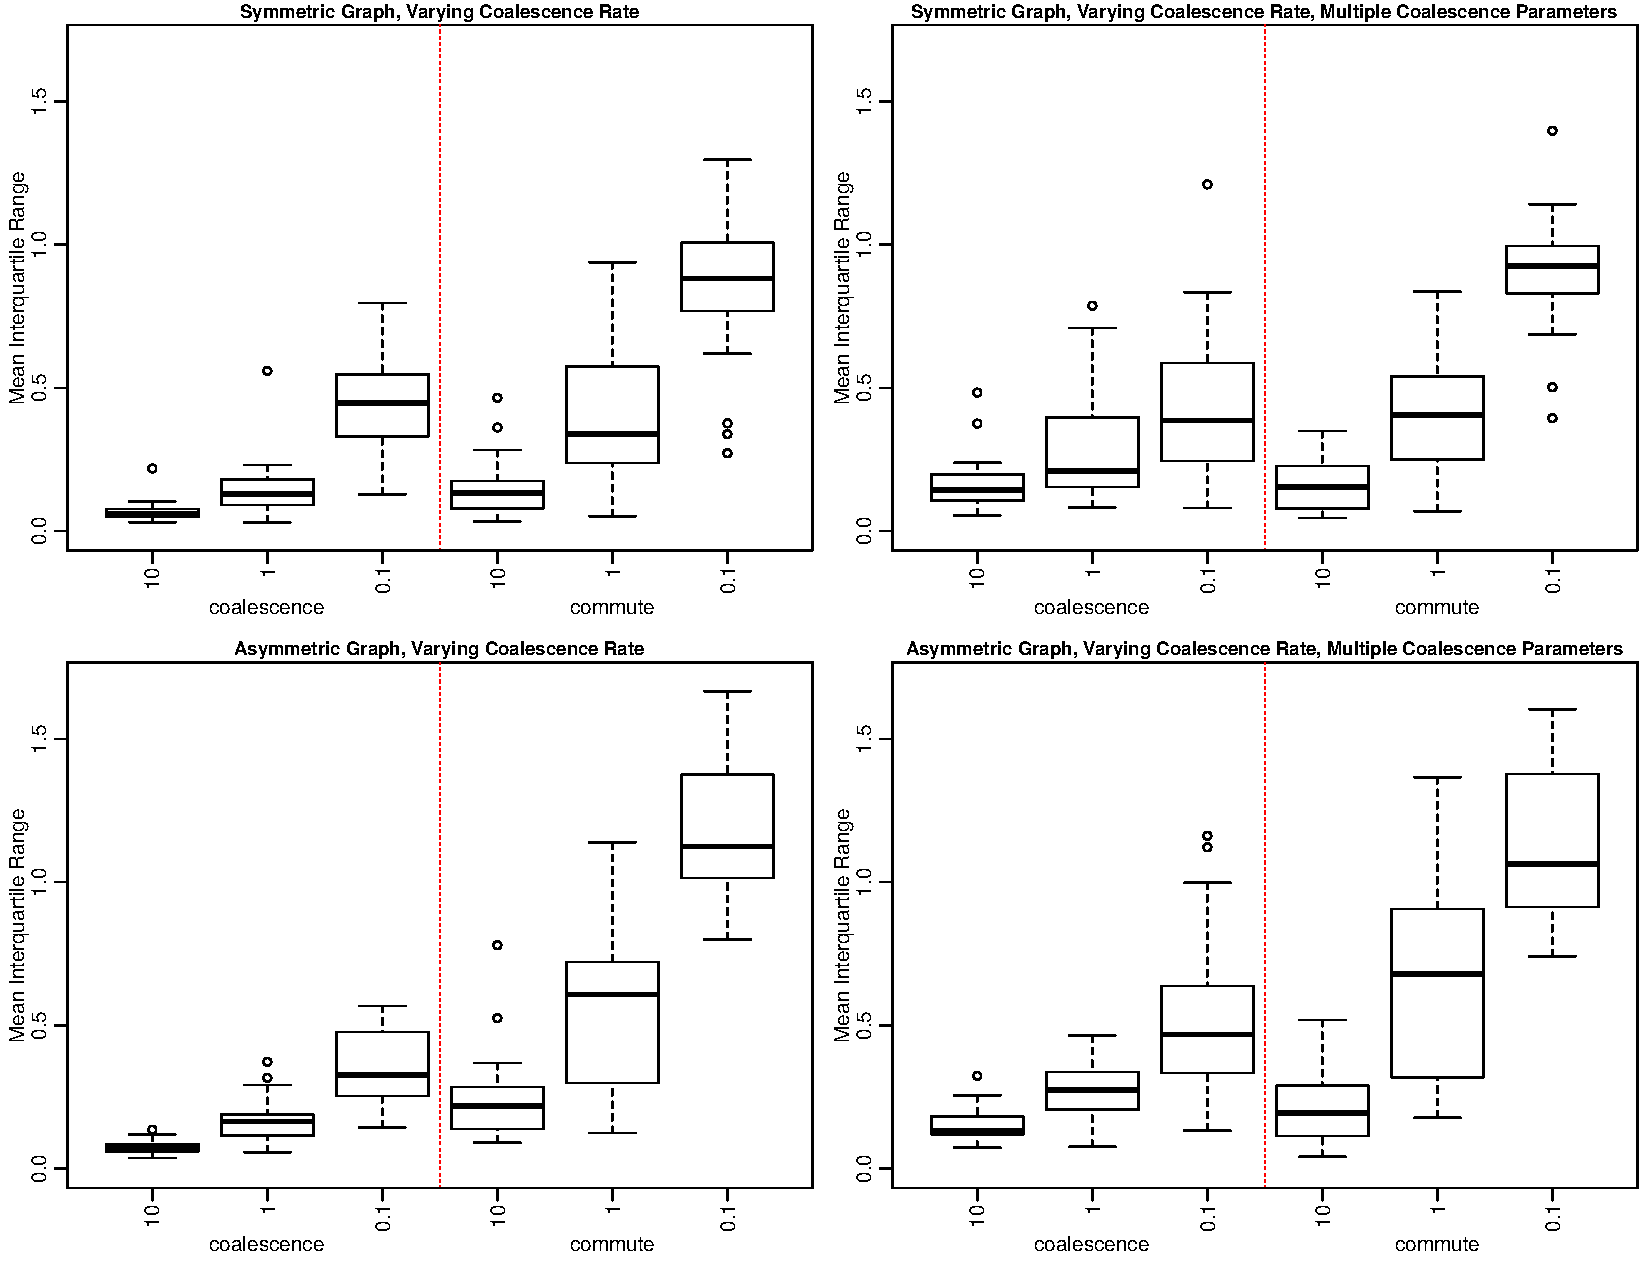
\includegraphics[scale=.6]{figs/mult_gam_iqr}
\caption{Boxplots of the mean interquartile ranges of the posterior distributions of $g$
for each of the 25 graphs in each situation.
Each box is labeled with the coalescence rate in the underlying model for each situation.
Subplot locations for each situation are the same as in Figure \ref{fig:mult_noise}.
%The top left shows the results for symmetric graphs 
%when there is a single coalescence parameter for all locations,
%the top right for symmetric graphs 
%when there is a separate coalescence parameter for each location,
%the bottom left for asymmetric graphs 
%when there is a single coalescence parameter for all locations,
%and the bottom right for asymmetric graphs 
%when there is a separate coalescence parameter for each location.
}
\label{fig:mult_gam_iqr}
\end{figure}


\begin{figure}
\centering
     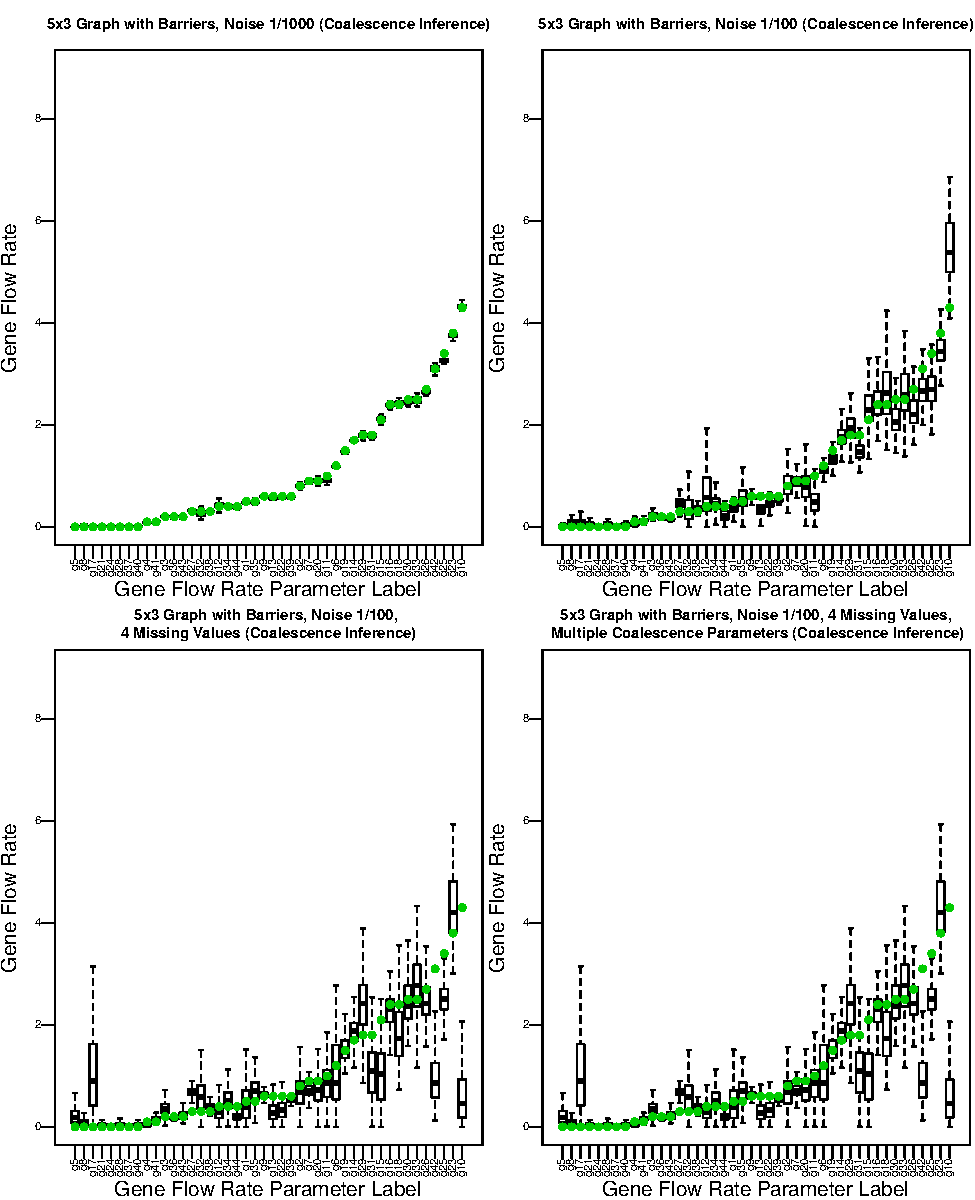
\includegraphics[scale=0.8]{figs/5x3boxplots}
    \caption{Posterior distributions for values of $g$ 
    for the 5 $\times$ 3 graph with barriers 
    for each of the analysis cases with coalescence time inference.
    See Figure \ref{fig:5x3b_grid} to see movement parameter locations.
    %\plr{TODO: put bottom two panels on top; on the bottom put the same thing for commute time}
}
    \label{fig:5x3boxplots_mult_gam}
\end{figure}


\begin{figure}
\centering
     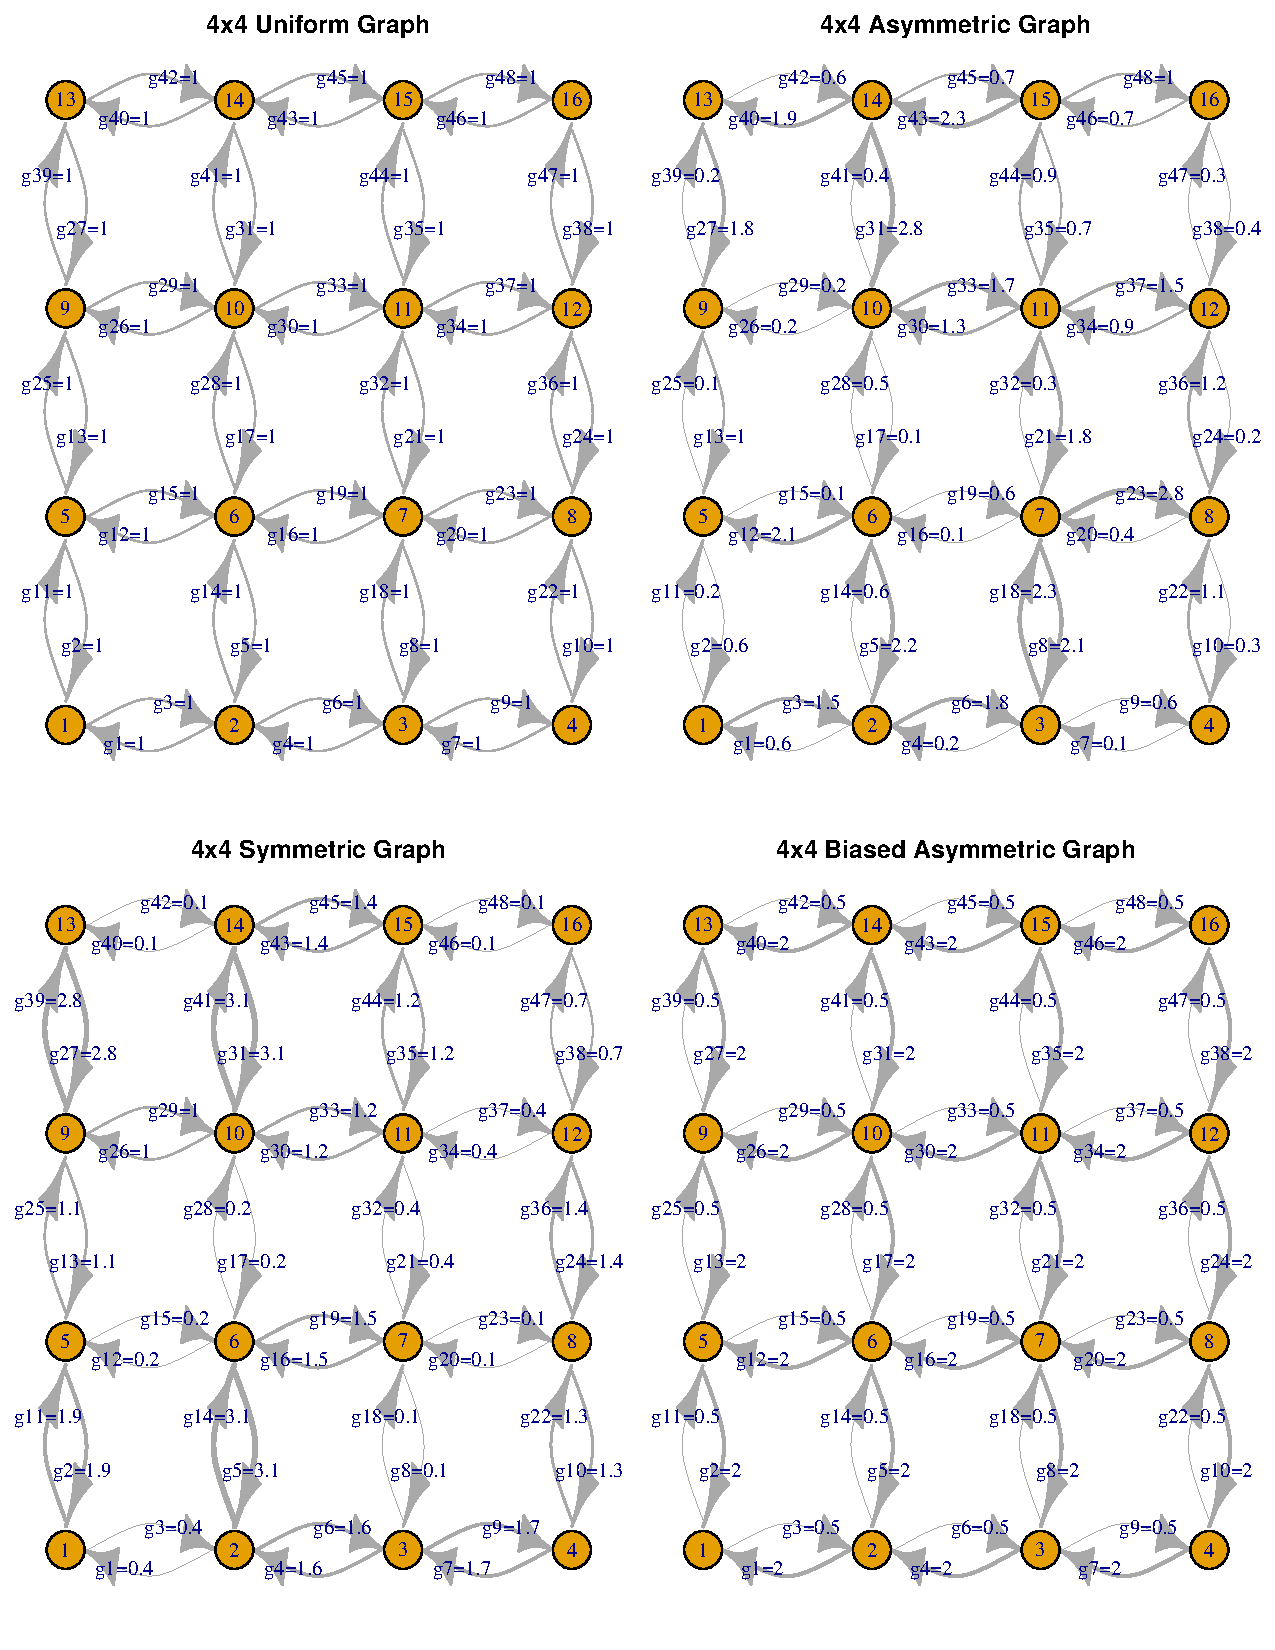
\includegraphics[scale=.8]{figs/4x4_grids}
    \caption{Plots of the grid structure 
    for the uniform graph, symmetric graph, the asymmetric graph,
    and the biased asymmetric graph 
    using the igraph R package.}
    \label{fig:4x4_grids}
\end{figure}


\end{document}
